\chapter{基于深度卷积网络的线虫前景轮廓分割}
\section{引言}
秀丽隐杆线虫由于通体透明,且PDMS制作的微流控芯片也是透明的,所以线虫轮廓的分割是个难点。
通过简单的阈值分割的方法,并不能够很好的分割线虫的轮廓,因为前景像素的灰度值范围被包括在背景像素的灰度范围内。
通过背景减除的方法分割的线虫轮廓。由于图像噪声的影响,会导致分割的线虫轮廓出现断裂、不完整等情况。
这些都会导致线虫跟踪的失败。另一方面,背景的估计需要$50\sim100$帧背景不变的图像。
当需要对线虫进行实时跟踪时,基于背景估计的线虫前景分割算法需要一个启动时间用于背景的估计。
另外,当CCD相机或载物台移动时(如:需要观察不同腔室中的虫子),由于背景的改变,这种算法还是会失效。
卷积网络作为一种强大的特征提取器在许多计算机视觉中取得了很大的成功。

	本课题将卷积网络用于线虫轮廓的前景提取具有如下优势:
	
\begin{enumerate}
  \item 与基于背景减除的方法相比,基于卷积网络的分割不需要对图像背景建模,只依赖当前帧的图像,从而能够保证实时性的要求。
  \item 能够降低硬件成本,传统的线虫图像处理,为了获得一个背景和线虫轮廓对比度比较高的图像。通常使用特制的硬件对CCD和照明都有很高的要求。卷积网络作为一种强大特征提取器降低了对图像质量的要求。
  \item 鲁棒性更好,传统的线虫轮廓分割算法,通常需要人工的选取一些超参数(如:分割的阈值,形态学操作中核的大小等等),但由于视频采集过程中照明的变化以及图像噪声的影响很难选取一个最佳的全局参数。
基于卷积网络的分割是一种端到端的方法,输出直接是分割的结果,因此,这种方法几乎不依赖超参数的选取,具有很好的鲁棒性。
\end{enumerate}

\section{线虫图像处理总体方案介绍}
	在介绍线虫前景轮廓分割之前,需要先介绍线虫图像处理的一般流程。如图\ref{fig:flow}所示,是本文提出的药物筛选
	平台线虫图像处理部分的总体流程,共分成4个阶段。第一个阶段是从采集到的视频中读取一帧图像,并将
	线虫轮廓覆盖的区域定义为前景,剩下的区域视为背景。这一阶段的输出为一幅二值化的图像,其中1表示前景0表示
	背景。如果是单线虫的跟踪,则第一个阶段的输出则为线虫的轮廓。但考虑到多线虫跟踪过程中多个线虫的轮廓会出现
	相交甚至纠缠在一起,导致因无法区分单个线虫轮廓从而跟踪丢失。第二个阶段的任务主要是对多个纠缠在一起的线虫轮廓进行解析,
	从而得到单个线虫的轮廓。第三个阶段的线虫跟踪是利用线虫轮廓的重心面积等信息找出相邻两帧图像之间线虫轮廓的对应
	关系。第四个阶段主要是利用跟踪到的线虫轮廓计算出线虫体长、运动速度和摆动频率等信息。本章主要介绍线虫图像处理流程中
	第一个阶段的内容。

	\begin{figure}[h]
	  \centering
	  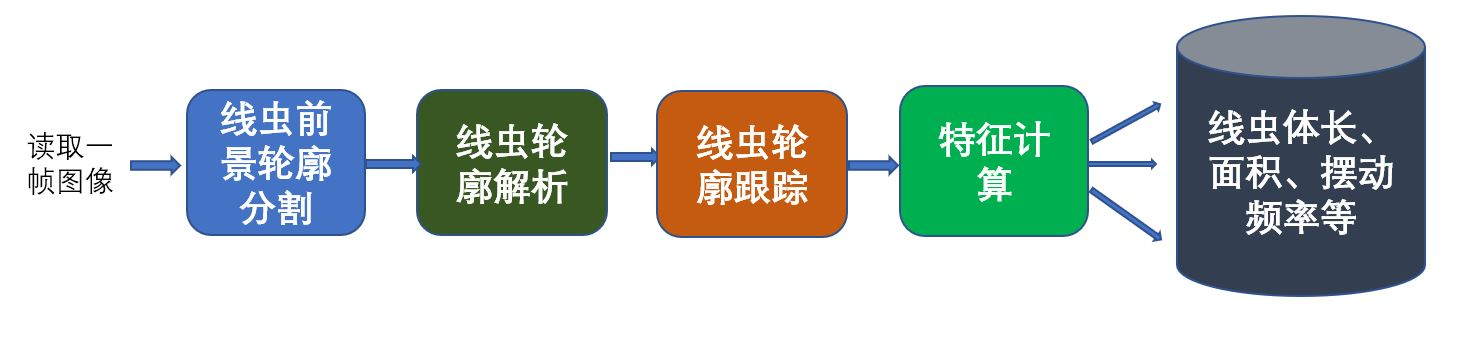
\includegraphics[width=14cm]{figure/chap3/flow.jpg}
	  % \hspace{1cm}
	  % 
\includegraphics[width=4cm]{example/sjtulogo.jpg}
	  \bicaption[这里将出现在插图索引中]
		{线虫图像处理总体流程图}
		{The flow chart of C.elegans image processing}
	  \label{fig:flow}
	\end{figure}
\section{传统的图像分割方法分类介绍}
	图像分割是生物医疗图像处理任务最重要的步骤之一,图像分割指的是将图像按照预先定义的
	相似度准则将图像划分为若干个区域的过程,相似度准则可以是代表同一个对象的像素
	的特性或特征。
\subsection{基于像素的图像分割方法}
	基于像素的阈值分割方法通过利用图像灰度直方图的统计信息来确定一个或者多个阈值,
	并对图像中每个像素进行比较和分类。其中OSTU于1979年提出了基于最大类间方差的阈值分割方法\cite{otsu1979threshold},
	通过最大化类间方差计算出一个全局最优阈值。与全局阈值法相对应的是自适应阈值的分割,由于每个像素的阈值
	是根据其局部邻域内的统计直方图计算的,所以对于光照不均匀的图像其具有很好的分割效果。除了以上提到
	的两种方法外,还有最大熵阈值法、双峰法、P参数法等。
	
	与通过阈值将像素分为多个类别的阈值分割方法不同,基于像素聚类的分割是通过对像素的灰度值或者特征
	向量的聚类实现图像分割。如彩色图像往往具有R、G、B三个通道,因此可以将每个像素的三个颜色通道的
	分量值添加到该像素的特征向量里。这是像素聚类的一个优势,其能够利用每个像素更多的信息,而阈值分割
	只能利用像素的灰度值。像素聚类往往产生不连续带有孔洞的区域或者具有单个孤立像素的区域,所以聚类后
	一般都需要后处理算法以消除这些缺陷。常用的后处理算法有区域生长、像素连接和一些基于规则的算法等。
	常见的聚类算法有K均值聚类算法\cite{forgy1965cluster}和以模糊集合为基础的Fuzzy cmeans(FCM)聚类聚类算法\cite{evers1999fuzzy}等。
\subsection{基于边缘的图像分割方法}
	基于边界的图像分割算法通常使用空间滤波的方法计算图像的一阶梯度和二阶梯度。Sobel算子、Prewitt算子
	和Robert算子常被用于
	计算图像的一阶梯度信息。Laplacian算子和Kirsch算子常被用于计算图像的二阶梯度信息。使用这些微分算子对图像进行空间滤波
	便可以将图像中不同区域的边缘检测出来。由于图像中噪声的影响,这些边缘通常是不连续的。
	为了形成闭合的区域,通常需要将这些不连续的边连接起来。常用的算法有Canny边缘检测算法。
\subsection{基于区域的图像分割方法}
	基于区域生长的图像分割方法是根据预先定义的相似性准则将相邻的像素或相邻的区域融合形成一个
	大的区域。当原图像被过度分割成很多小区域时,区域生长的方法作为一种有效的后处理方法能够处理分割
	过程中目标轮廓出现断裂的情况。与区域生长相对应的是区域分裂,这种方法可以将一个大的区域分割成两个
	或者更多的小区域。另外,区域分裂的分割方法可能使目标轮廓产生孔洞。
\subsection{交互式的图像分割方法}
	所谓交互式的图像分割方法指的是需要用户提供输入的分割方法(如:需要用户提供一个矩形框或者鼠标点击
	等输入操作),是一种半自动化的图像分割方法。目前常见的交互式图像分割方法有基于图论的GrabCut算法\cite{rother2004grabcut}
	和基于曲线演化的活动轮廓分割方法\cite{kass1988snakes,tsai2001curve}。GrabCut算法是由Rother等人于2004年提出,通过引入Gibbs能量函数,将前景背景分割
	问题转化为一个能量最小化的问题,通过迭代计算的方式将能量最小化。在分割的过程中,用户还可以用画刷将某个区域标记为前景或
	背景,然后让算法基于已经分割的结果继续迭代以改善分割的性能。另一方面,基于活动轮廓的分割方法总是能够获得连续的闭合的轮廓。
	特别是将水平集理论应用于活动轮廓分割使得该方法可以自动处理轮廓的分裂和合并,使其更具灵活性。其原理
	是曲线在某些力的联合作用下呈现扩张或者收缩的运动,最终会收敛于目标轮廓的边缘。但是活动轮廓的分割方法需要
	提供一个初始轮廓作为算法的输入,因此也是一种半自动化的图像分割算法。
\subsection{基于背景减除的分割方法}
	Zivkovic等人\cite{zivkovic2006efficient}在2006年提出了一种基于对单个像素进行混合高斯建模的背景估计的方法。
	其主要针对背景固定的视频。以上小节提到的分割方法都只需要用到当前帧图像的信息,而与上面提到的分割算法不同,基于背景减除的分割方法还需要用到当前帧之前的
	多帧图像信息。对图像中每一个像素用一个混合高斯概率函数建模。模型参数包括高斯均值$u_i$、高斯方差$\sigma_i$、高斯权重$w_i$。每读取
	一帧图像,便对模型做一次更新。预测背景的时候,将所有高斯按照其权重的大小排序,取前$B$个高斯分量作为背景,$B$由
	公式\ref{eq:gmm}表示,其中参数T表示背景所占的比例。得到每一帧图像的背景后再与当前帧图像相减,经过二值化处理
	后便可得到分割后的前景轮廓。
	\begin{equation}
	B=\mathop{\arg\min}_{b} \sum_{k=1}^b w_k>T \label{eq:gmm}
	\end{equation}
\section{卷积神经网络介绍}
	从1956年正式提出人工智能学科以来,人工智能领域的研究经历了60年的发展。期间,不同学科背景的学者们对人工智能的实现,提出
	了不同的观点并由此产生了不同的学术流派。其中对人工智能领域影响较大的主要有符号主义(Symbolism)、
	连接主义(Connectionism)和进化主义(Evolutionism)或控制论学派(Cyberneticsism)等。
	目前,在诸多领域取得重大突破的深度学习(Deep learning)技术是连接主义学派的典型代表性技术。其主要受
	神经科学的启发,大脑中大量的神经元形成复杂的连接,信号在神经元之间传递。人工神经网络(Artificial Neural Network,ANN)
	利用大量相互连接的节点构成,每个节点代表一个特定激活函数的输出,每两个节点之间的连接都有一个权重。通常,神经网络模型
	都是由多层网络堆叠而成,前一层网络的输出作为后一层网络的输入。从网络的输出来看,整个网络的输出相当于由许多张量函数嵌套构成的
	复合函数,网络模型参数的训练依赖的误差反向传播算法其实质是复合函数的链式求导法则。
	
	卷积网络(Cnvolutional Neural Network,CNN)是人工神经网络模型中的一种,由Yan Lecun于1989年提出并将其用于手写数字识别
	\cite{le1989handwritten},卷积操作类似于图像处理中的空间滤波,与之不同的是滤波核作为模型参数是通过学习得到的。
	一个典型的卷积网络架构如图\ref{fig:chap4:cnn}所示,通常由卷积层,池化层,全连接层等构成。为了使模型具有更好的泛化
	性能,通常在不同的层之间还会加入Dropout层和Batch Normalization层。自2006年以来,研究者们不断对卷积网络进行改进提出
	了很多性能优异的网络架构(如:AlexNet网络\cite{krizhevsky2012imagenet}、VGG网络\cite{simonyan2014very}、
	GoogLenet网络\cite{szegedy2015going}和ResNet网络\cite{Kaiming2015Deep})。使卷积网络在许多计算机视觉任务中大放异彩。
	\begin{figure}[h]
	  \centering
	  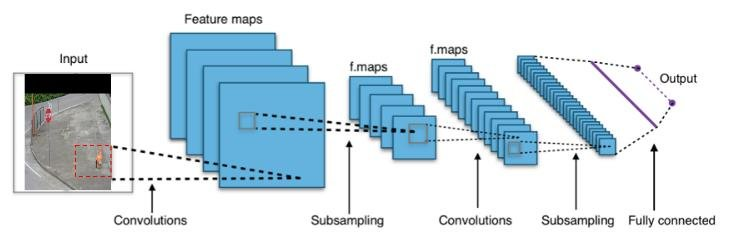
\includegraphics[width=12cm]{figure/chap4/CNN-arch.png}
	  \bicaption[这里将出现在插图索引中]
		{卷积网络的经典结构}
		{A typical architecture of CNN}
	  \label{fig:chap4:cnn}
	\end{figure}
\subsection{卷积层}
	卷积层是卷积网络中主要的连接层,由于其引入权值共享的机制,与全连接的方式相比将网络的模型参数减小了几个数量级,
	且对输入图像的缩放和旋转等变形具有高度不变性。如图\ref{fig:chap4:cnn-op}所示,卷积操作可以理解为卷积核在输入
	张量上的滑动。输出张量的尺寸大小由卷积核的大小、填充的大小、步长和输入张量的大小决定。
	公式\ref{eq:cnn:io}表示了这一关系,其中$o$和$i$表示输出张量和输入张量在某一维度的大小,$p$和$s$分别表示
	填充的大小和卷积步长,k表示卷积核的大小。图\ref{fig:chap4:cnn-op}中$i=6,p=1,k=3,s=2$根据公式\ref{eq:cnn:io}
	可以得到$o=3$。
	\begin{equation}
		o = \lfloor \frac{i+2p-k}{s} \rfloor +1 \label{eq:cnn:io}
	\end{equation}
	
	\begin{figure}[h]
	  \centering
	  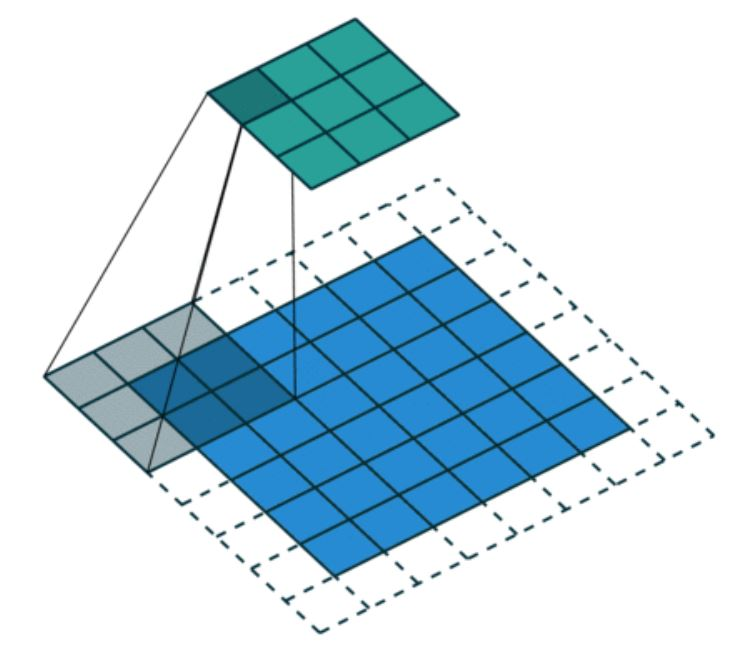
\includegraphics[width=7cm]{figure/chap4/CNN-op.jpg}
	  \bicaption[这里将出现在插图索引中]
		{卷积操作示意图}
		{Convolution operation diagram}
	  \label{fig:chap4:cnn-op}
	\end{figure}
\subsection{池化层}
	池化层是一种对输入张量进行降采样的操作,由于其是在输入张量的每一个通道上进行的,所以不会改变通道的数目。
	池化操作可以大致分为最大值池化、均值池化和随机池化三种,
	其都是通过对输入张量一个邻域内的像素值进行聚合统计实现的。因为部分像素的改变并不会对聚合统计的结果
	造成太大的差异,因此池化操作具有一定的尺度不变性。如图\ref{fig:pooling}是三种池化操作的示意图,最大值
	池化求领域内特征点的最大值作为统计输出,均值池化求领域内特征点的平均值作为统计输出,随机池化将领域内
	特征点按照其数值大小赋予概率,然后按概率采样得到结果作为统计输出。
	\begin{figure}[h]
	  \centering
	  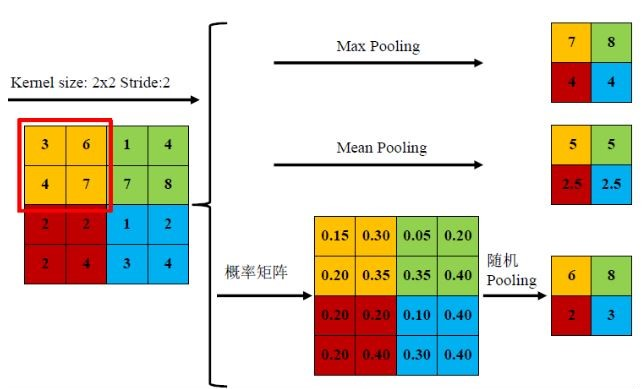
\includegraphics[width=8cm]{figure/chap4/pooling.jpg}
	  \bicaption[这里将出现在插图索引中]
		{三种池化操作示意图}
		{Three pooling operations diagram}
	  \label{fig:pooling}
	\end{figure}
\subsection{Dropout层}
	为了解决神经网络过拟合的问题,Srivastava和Hinton等人\cite{srivastava2014dropout}于2014年提出dropout
	方法,有效的提高了网络的泛化能力。如图\ref{fig:dropout-connection}所示,在网络训练阶段,对每一个神经元以一定的概率
	丢弃。从而每次更新网络权值时,网络的连接都是随机的,相当于对采样到的网络进行更新。在网络测试阶段,为了
	得到所有随机连接网络的平均输出,这个阶段网络使用全连接的方式并且将网络的权值以一定的比列缩放。大量的实验表明,
	采用Dropout的网络具有很好的泛化能力且能够加速网络的收敛。
	\begin{figure}[!htp]    
\begin{minipage}[t]{0.5\linewidth}%设定图片下字的宽度,在此基础尽量满足图片的长宽    
	\centering    
	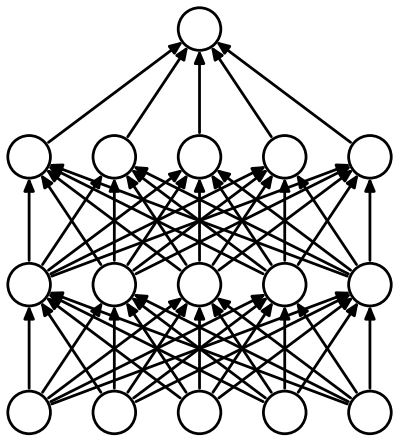
\includegraphics[width=0.9\linewidth]{figure/chap4/no-dropout.jpg}    
	\caption*{(a) 测试阶段网络连接 }
	\label{fig:no-dropout}    
\end{minipage}    
\begin{minipage}[t]{0.5\linewidth}%需要几张添加即可,注意设定合适的linewidth    
	\centering    
	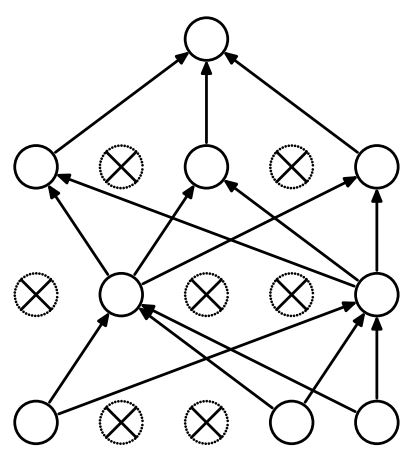
\includegraphics[width=0.9\linewidth]{figure/chap4/dropout.jpg}    
	\caption*{(b) 训练阶段网络的连接}
	\label{fig:dropout}
\end{minipage}
\bicaption{Dropout神经网络模型}{Dropout Neural Net Model.}%n张图片共享的说明
\label{fig:dropout-connection}
\end{figure}

\subsection{Batch Normalization层}
	批量标准化(Batch Normalization,BN)是深度学习领域一种非常重要的正则化的方法\cite{ioffe2015batch},有效的
	解决了内部方差偏移(Internal Covariate Shift)的问题。内部方差偏移指的是在网络训练的过程中,隐藏层的输入的
	分布一直在变,导致网络收敛变慢。批量标准化的方法可以使隐藏层的输入分布稳定并近似分从标准正态分布,很多
	激活函数(如tanh函数和sigmoid函数等)在0值附近的梯度是最大的,因此可以获得一个较大梯度,从而大大提高了网络的训练速度。
	另外,还降低了对初始学习率选取的敏感度。
\section{线虫轮廓前景分割卷积网络的设计及模型评估}

\subsection{数据集的制作}
\subsubsection{数据集的采集}
	图\ref{fig:chap5:camera}是线虫图像采集的系统装置图,主要由显微镜、CCD相机、照明系统和微流控芯片四个部分组成,CCD
	相机通过数据线连接电脑进行图像数据传输。线虫通过注射泵注入到微流控芯片的腔室内。移动显微镜的载物台使线虫腔室
	位于视野的正中央。调节显微镜的放大倍数使线虫腔室充满整个视野。调整显微镜焦距使视野中呈现清晰的图像。调整CCD相机的
	曝光时间以获得一个对比度比较高的线虫图像。完成以上步骤后便可以进行线虫视频的录制。
	\begin{figure}[thb]
	  \centering
	  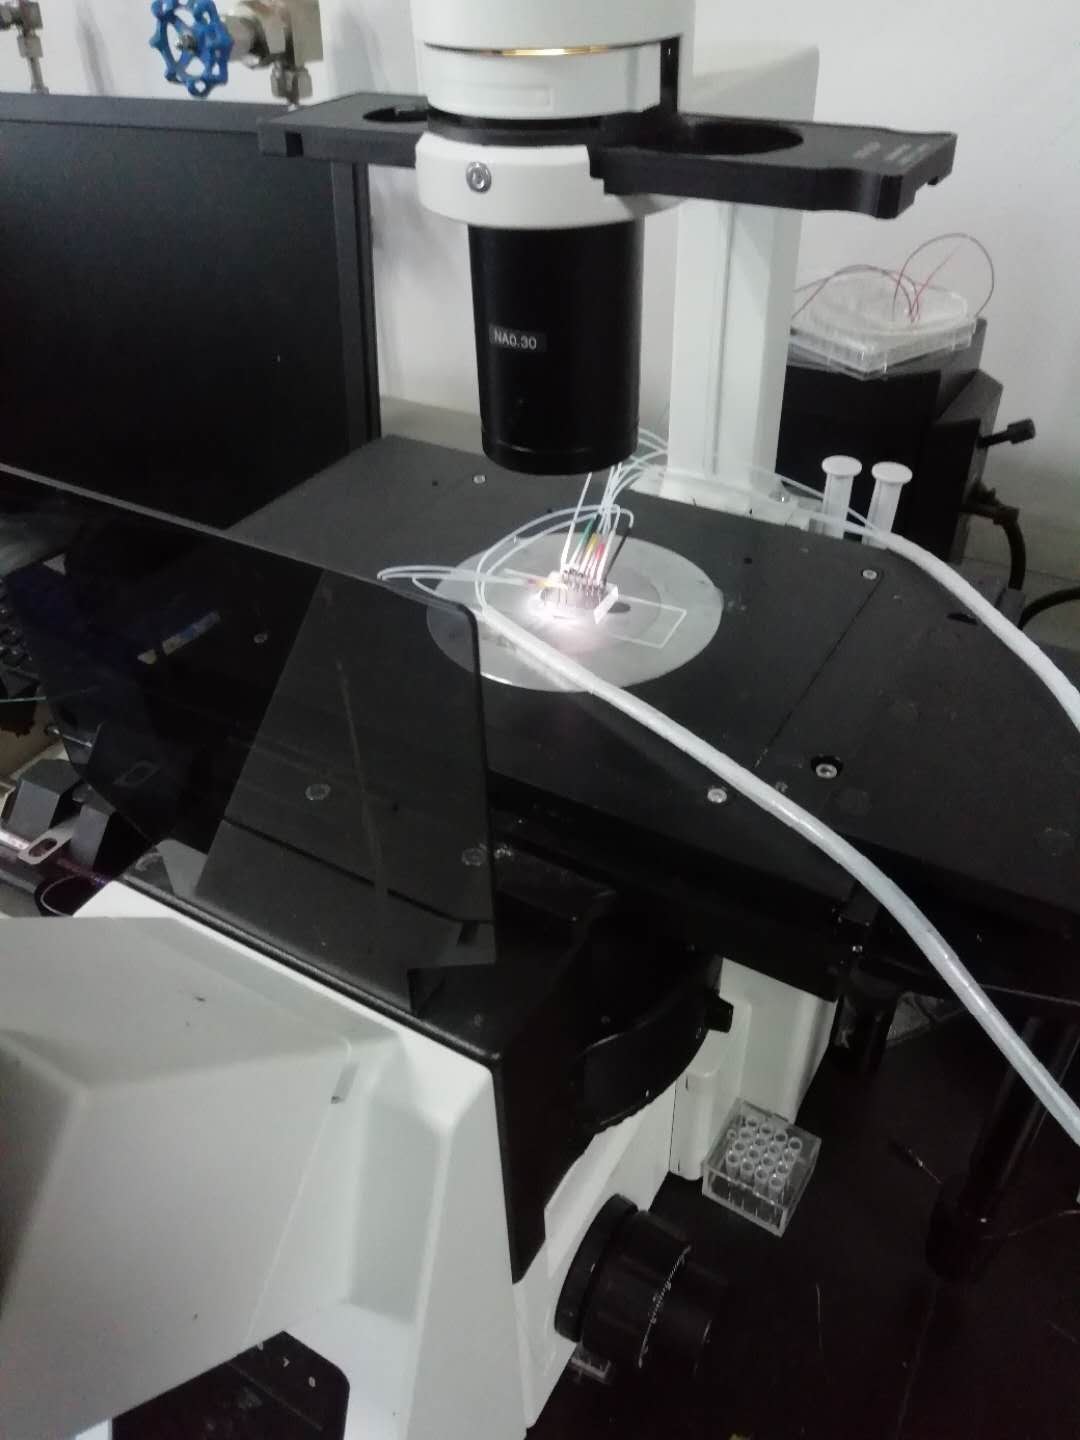
\includegraphics[width=8cm]{figure/chap5/camera.jpg}
	  \bicaption[这里将出现在插图索引中]
		{图像采集系统装置图}
		{System diagram of image acquisition}
	  \label{fig:chap5:camera}
	\end{figure}
\subsubsection{数据集的标注}
	高质量的数据集对网络的训练来说至关重要,且数据集的质量决定了神经网络模型性能的上限,通过优化网络架构的方法
	也只能逼近这个上限。但数据集的标注通常是一个非常耗时的过程,特别是图像分割任务要对不同的区域标记。目前很多的
	图像分割标注工具(如:Labelme\footnote{\url{https://github.com/wkentaro/labelme}}和Ratesnake\footnote{\url{https://is-innovation.eu/ratsnake/}}等)都是采用多边形近似的标注方法,
	即在轮廓的四周边缘采集足够多的点,这些点构成的多边形为标注对象的轮廓。由于线虫形态变化复杂,相对于其他目标
	的标注往往需要采集更加密集的点才能满足线虫轮廓标注的精度。为了提高线虫图像标注的效率,本文采用了一种半自动的线虫轮廓
	标注方法。将Grabcut算法用于线虫轮廓的标注,只需要用矩形框将线虫轮廓框出作为Grabcut算法输入,算法可以自动的分割
	出线虫的轮廓,最后再将多个线虫轮廓合成为一个标签图像。通过这种方法,本文制作了一个包含236个样本的数据集,图\ref{fig:dataset}是数据集部分示例。
	整个数据集按照$8:2$的比例将其分为训练集与测试集两部分分别用于网络模型的训练与测试。
	\begin{figure}[h]
	  \centering
	  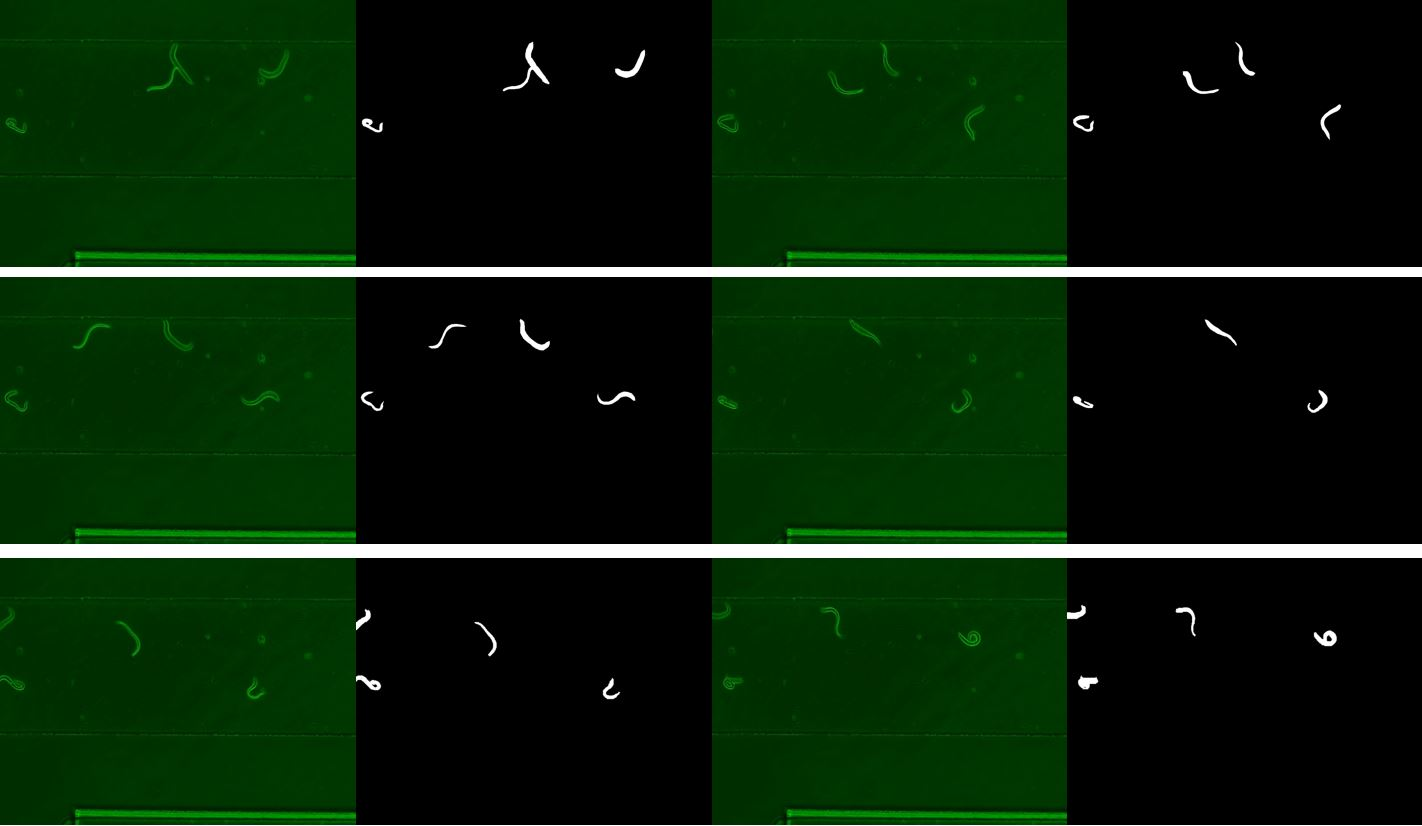
\includegraphics[width=14cm]{figure/chap3/dataset.jpg}
	  % \hspace{1cm}
	  % 
\includegraphics[width=4cm]{example/sjtulogo.jpg}
	  \bicaption[这里将出现在插图索引中]
		{线虫前景轮廓分割数据集示例}
		{The image examples from C.elegans foreground segmentation dataset}
	  \label{fig:dataset}
	\end{figure}
\subsection{条件随机场模型在分割任务中的应用}
	条件随机场(Condition random field, CRF)是概率无向图模型中的一种\cite{李航2012统计学习方法},
	目前被很多研究者用于解决图像分割问题并取得了很大的成功\cite{zheng2015conditional,wang2017adaptive,chen2018deeplab}。
	其能够对空间中相邻像素之间的关系进行建模,从而可以得到具有空间一致性和更加精细化的分割结果。
	如果分割算法没有考虑到相邻像素之间的依赖关系,相当于认为空间中每个像素都是独立的,
	这样会导致分割结果中被分割对象的不连续以及可能丢失掉很多细节结构。本文将条件随机场模型应用于
	线虫前景轮廓的分割任务中,并通过卷积模块加以实现,这样可以保证整个模型的可微性。
		
	线虫图像的前景背景分割问题本质上是一个二分类问题,假设有一个标签$Y=\{Y_1,Y_2,\cdots,Y_N\}$
	,$N$表示总的像素,$Y_i\in\{0,1\}$则标签$Y$总共有$2^N$种取值。在$Y$的所有取值中,概率最大对应的取值
	即为最优分割的结果。图像分割问题被转化为基于条件随机场的最大条件概率问题。根据吉布斯分布与条件随机场
	的等效性\cite{Lafferty2001Conditional},定义如下基于标签$Y$的能量函数:
	\begin{equation}
		E(Y|I) = \sum_{l}Y_lU(l)+\sum_{l,k}Y_lW_{l,k}Y_k
	\end{equation}
	其中一元项$U(l)=g(h,l)$表示第$l$个像素标签$Y_l$取值为1的损失,$h$表示图像特征,$W_{l,k}$表示标签$Y_l$和
	标签$Y_k$同时出现的权重。给定一幅线虫图像$I$,对应的标签为Y的条件概率为:
	\begin{equation}
		P(Y|I)=\frac{1}{Z}\exp(-E(Y|I))
	\end{equation}
	其中$Z$为归一化项。通过平均场近似\cite{zheng2015conditional}的方法,标签$Y_l=1$可以通过以下迭代的方法求出:
	\begin{equation}
		\Phi(Y_l=1)_t=\sigma\Big(U(l)+\sum_{k}W_{l,k}\Phi(Y_k=1)_{t-1}\Big)
	\end{equation}
	其中$\Phi(Y_l=1)$表示$Y_l$取值为1的概率,$\sigma(a)=1/(1+\exp(-a))$表示 sigmoid 函数。$U(l)$通过基于图像特征$h$的卷积获得。
	$\sum_{k}W_{l,k}\Phi_{t-1}$是通过$t-1$阶段的概率图$\Phi_{t-1}$与卷积核$W$的卷积操作实现的。在$t$时刻的概率图$\Phi_t$可以由如下公式计算:
	\begin{equation}
		\Phi_t=\mathscr{M}(U,W^k)=\begin{cases}
						\sigma(W^k*U), \quad \quad \quad t=0\\
						\sigma(W^k*\Phi_{t-1}+U), \quad t=1,2,3
						\end{cases}
	\end{equation}
	其中$\mathscr{M}$表示基于共享权重的递归卷积,$W^k$表示共享卷积核,主要用于对相邻像素之间的空间
	关系进行建模。本文中,我们使用了3次递归卷积实现条件随机场的近似。
	
	
\subsection{网络结构的设计}
	本文提出了一种用于线虫前景轮廓分割的基于条件随机场的卷积网络模型,图\ref{fig:chap5:arch}为对应的网络架构。
	融合多种尺度的信息对分割任务来说是相当重要的(如:U-net网络\cite{ronneberger2015u}和SegNet网络\cite{badrinarayanan2015segnet}架构的设计),
	充分利用不同尺度的信息能够提高目标的定位精度从而减小分割误差,本文在分割网络架构的设计上也结合了多种尺度的
	信息。在图\ref{fig:chap5:arch}中,网络的前半部分通过降采样操作引入新的分支,网络的后半部分通过上采样操作并与
	上游的分支融合。网络输入张量的尺寸为$592\times800\times3$(代表一幅RGB彩色图像),通过不断分支并降采样,网络
	在最底层的分支上达到最小尺度(分辨率为:$37\times50$)。每次降采样都将分辨率降低为原来的一半,同时将特征通道数数扩大为
	原来的两倍。最终网络与最上层的分支融合得到尺寸为$592\times800\times16$特征图,将特征图与上一章节介绍的条件随机场
	模块相连接构成整个分割网络的结构。
	\begin{figure}[thb]
	  \centering
	  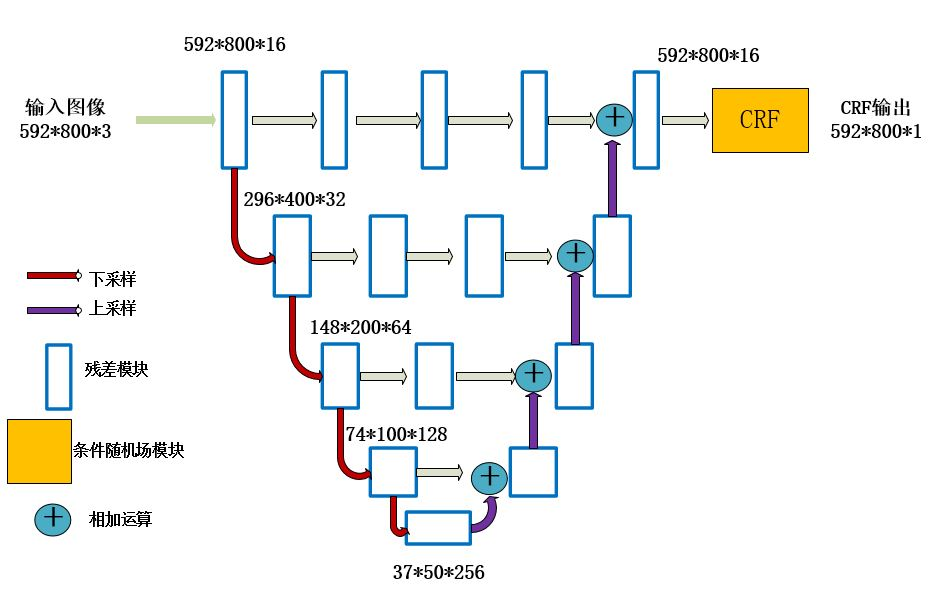
\includegraphics[width=13cm]{figure/chap5/arch.jpg}
	  \bicaption[这里将出现在插图索引中]
		{分割网络架构图}
		{The Architecture of segmentation network}
	  \label{fig:chap5:arch}
	\end{figure}
	\begin{figure}[htb]
	  \centering
	  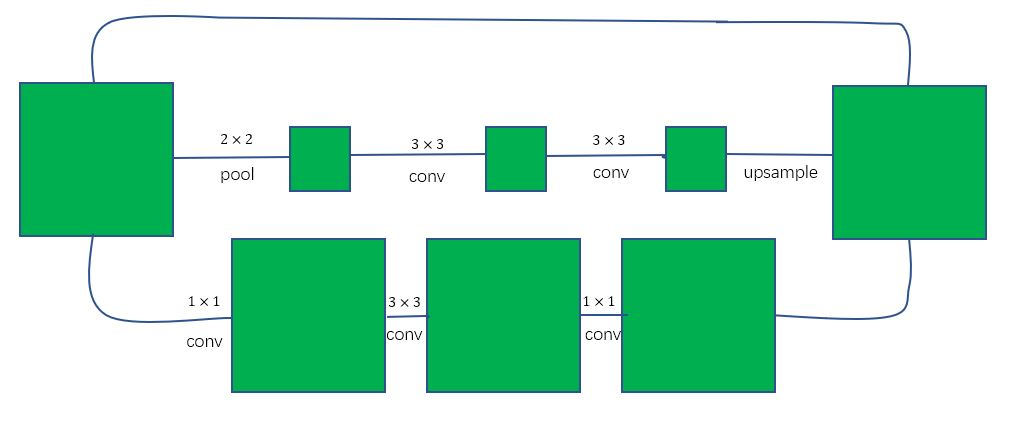
\includegraphics[width=9cm]{figure/chap4/residualpooling.jpg}
	  \bicaption[这里将出现在插图索引中]
		{残差连接模块}
		{Residual connection module}
	  \label{fig:chap4:respool}
	\end{figure}
	残差网络\cite{he2016deep}能够在增加网络深度的同时使网络依然易于训练,更深的网络往往能够学习到
	更加抽象的特征从而提高网络的性能。因此本文使用了如图\ref{fig:chap4:respool}所示的残差连接模块\cite{chu2017multi},这种残差
	模块包含三个连接通路。中间的通路由于使用了降采样,在卷积核尺寸保持不变的情况下,输出神经元的感受野将扩大到原来的两倍。
	但由于使用了降采样,所以导致分辨率下降。但上下两条路径上包含高分辨率的信息。最后将这三个路径的输出叠加在一起作为残差
	连接模块的输出。这种连接方式在扩大网络的感受野的同时依然保持原来的分辨率。
	
\subsection{网络模型的训练}
	在线虫的实时跟踪任务中,神经网络模型的复杂度和实时性是需要关注的重点。太复杂的网络其推断时间耗时太长往往达不到
	实时性的要求,因此必须要在网络结构的选取时加以考虑。而网络的训练和推断所消耗的时间的评估依赖于所采用的机器学习库
	和网络模型运行的硬件平台。因此为了评估不同网络模型的复杂度和实时性,表\ref{tab:hardwareconfig}
	列出了本文中所有网络模型运行的硬件平台。
	\begin{table}[!hpb]
	\centering
	\bicaption[指向一个表格的表目录索引]
    {算法运行的实验平台}
    {Experimental platform for algorithm running}
	\label{tab:hardwareconfig}
	\begin{tabular}{p{80pt}p{100pt}}
	\toprule
	平台参数 & 配置 \\
	\midrule
	操作系统 & Windows 10 家庭版\\
	系统内存 & 8g \\
	CPU & i5-6300HQ \\
	GPU & GTX 950M \\
	显存 & 4g \\
	深度学习库 & Tensorflow \\
	\bottomrule
	\end{tabular}
	\end{table}
	
	增强训练数据的多样性能够有效提高网络的泛化性能,特别是在较小的数据集上网络可能会出现过拟合的情况。为了
	提高网络的泛化能力,在网络训练阶段本文对训练集进行了数据增强。本文首先对训练图片以一定概率随机地进行水平镜像翻转或
	垂直镜像翻转,并将对应的标签做相同的变换。最后将训练图片加入一定量的高斯白噪声,以提高数据的多样性。
	在batchsize参数的选择上,考虑到本文训练图片的分辨率较高(为$592\times800\times3$)以及
	网络训练采用的硬件GPU显存较小(4g),因此不能将batchsize设置过大,本文这里将batchsize设为1,即采用单样本
	更新的方式训练网络。假设网络的最后一层输出是一张概率图设为$\Phi$,$y$为标签图(只包含0和1)。
	公式\ref{eq:loss}表示网络训练的交叉熵损失,通过随机梯度下降的方式不断的调整网络的模型参数使交叉熵损失不断下降。
	最终网络收敛到局部极小值或者全局最小值,训练损失将不会再下降。图\ref{fig:train_progress}表示训练过程中,训练
	损失和像素准确率随迭代次数的变化。图中可以看出随着迭代次数的增加,训练损失不断减小,像素正确率不断增加。网络在第
	1000次迭代后,网络基本已经收敛。
	\begin{equation}
		entropy\_loss = \sum_{i,j}y_{ij}\log \Phi_{ij} + (1-y_{ij})\log (1-\Phi_{ij}) \label{eq:loss}
	\end{equation}
	
	\begin{figure}[!htp]    
	\begin{minipage}[t]{0.5\linewidth}%设定图片下字的宽度,在此基础尽量满足图片的长宽    
		\centering    
		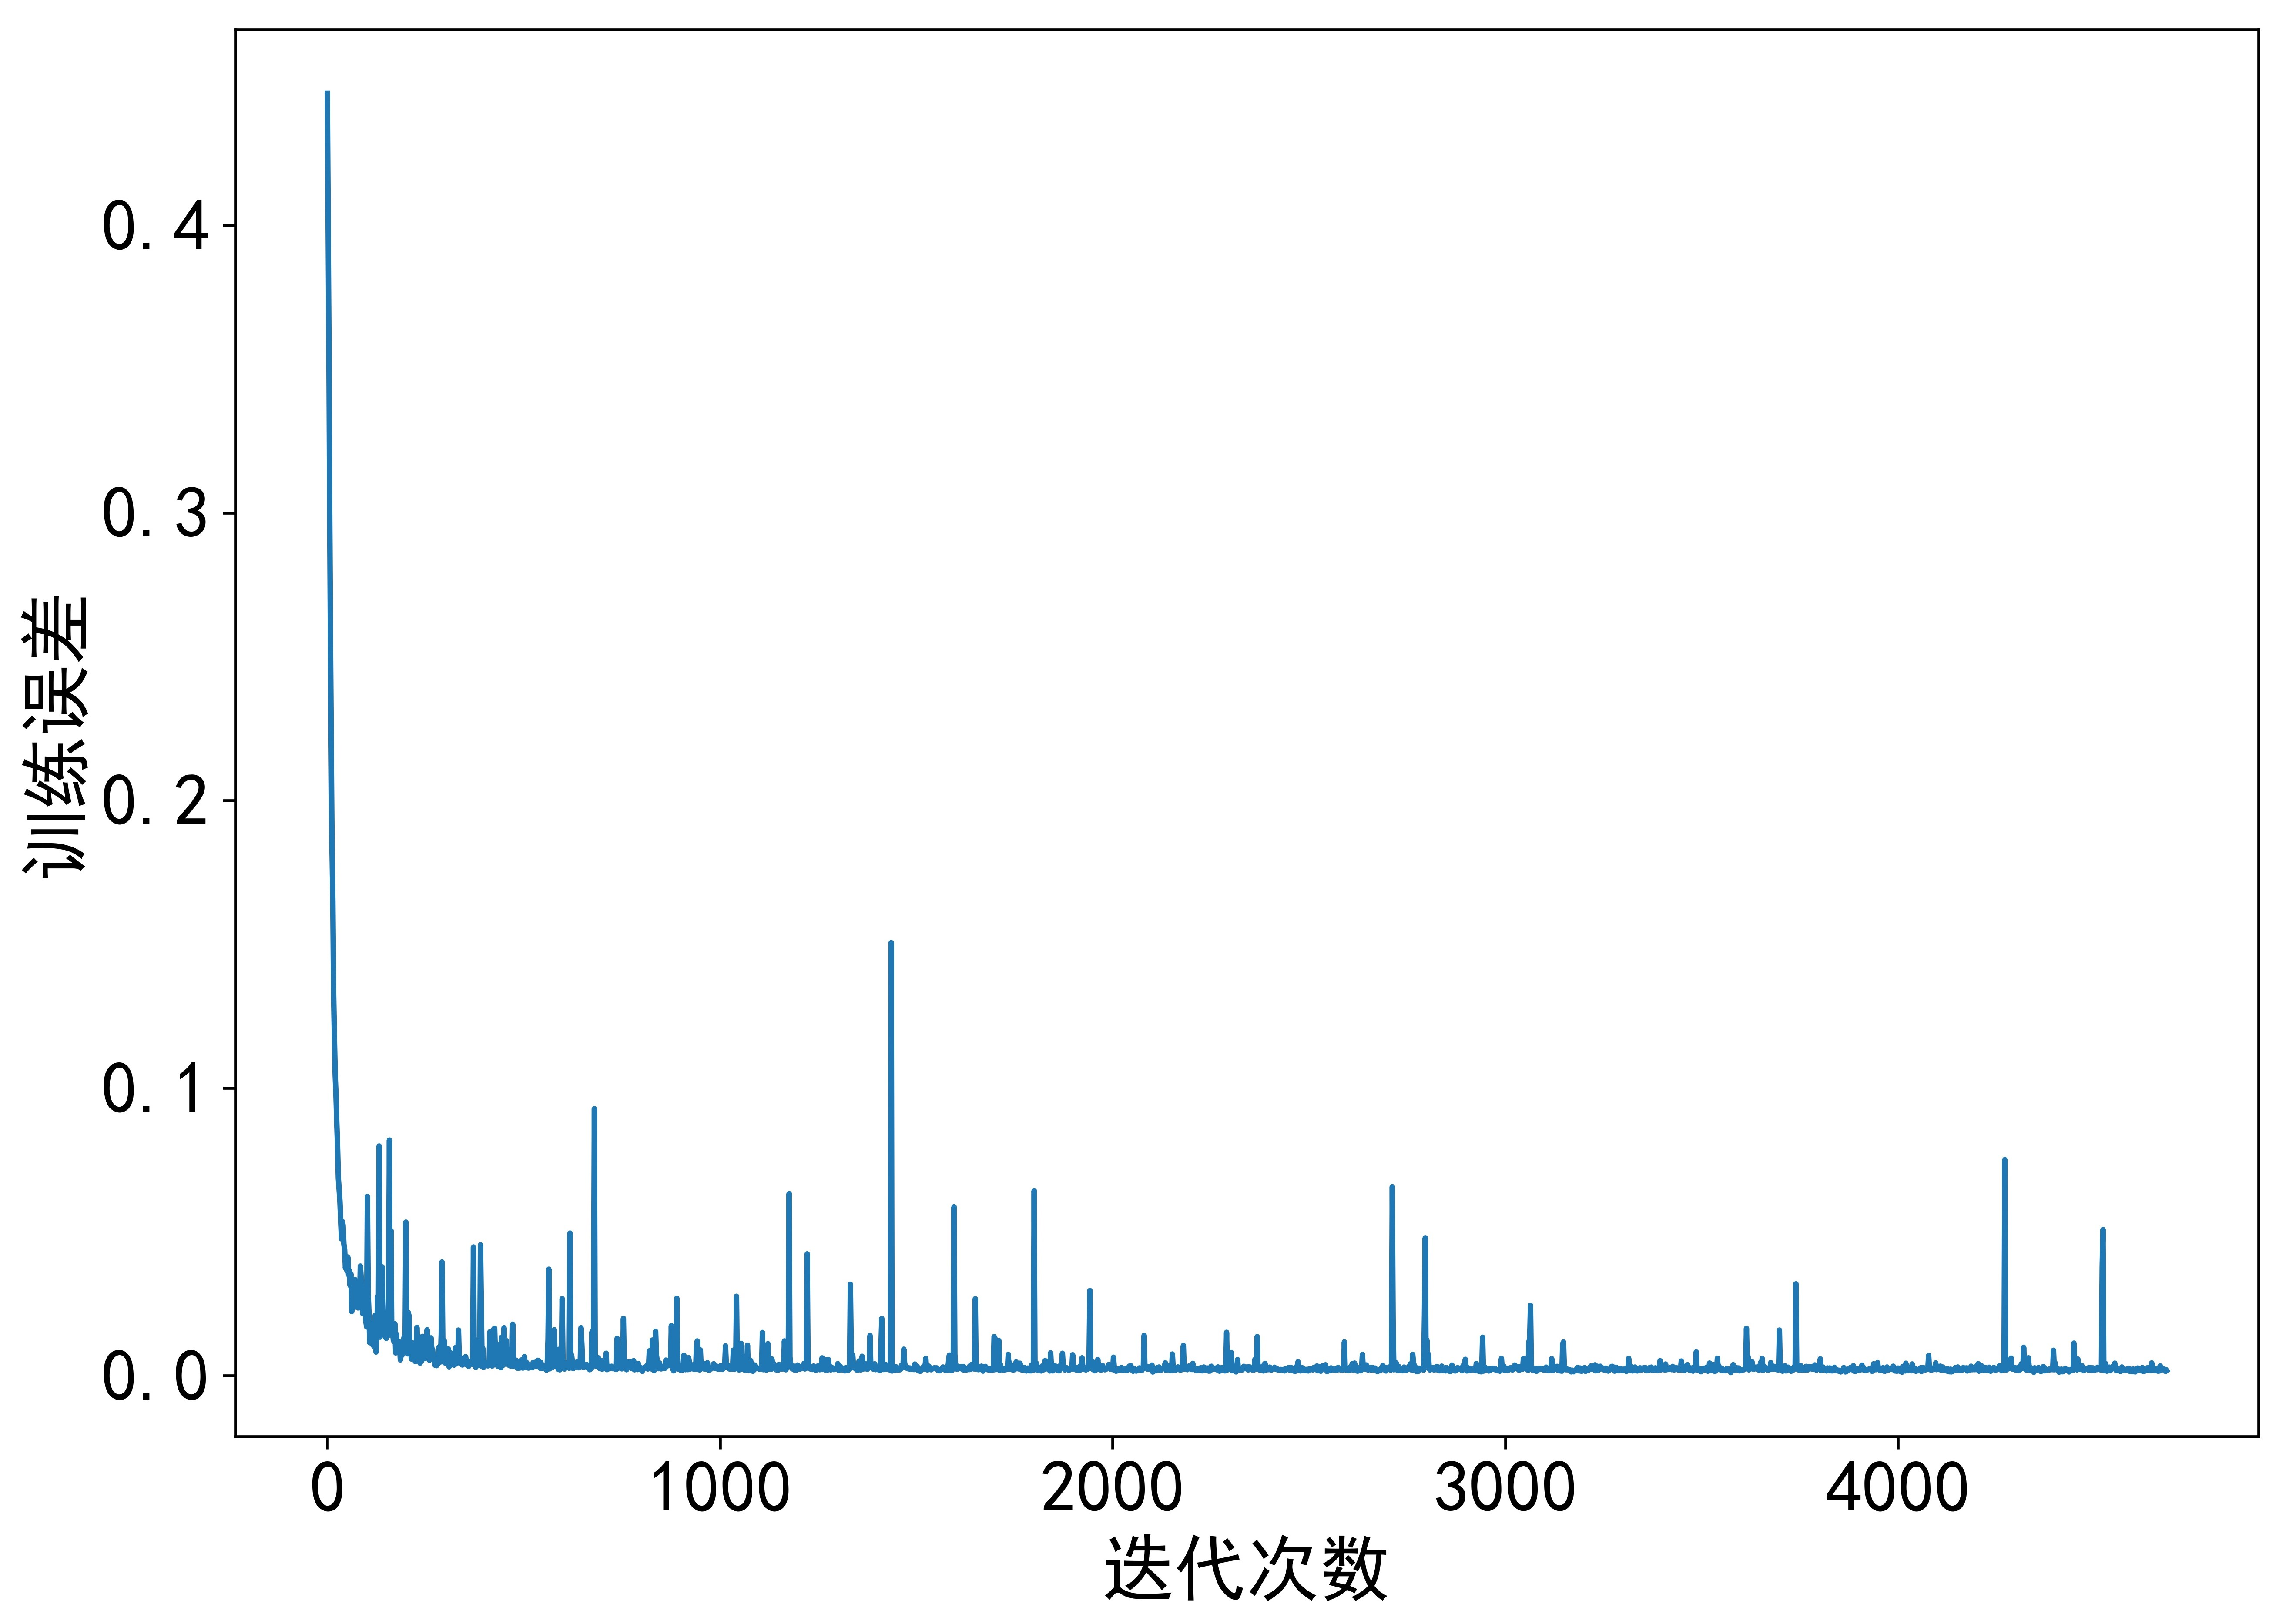
\includegraphics[width=1\linewidth]{figure/chap3/loss.jpg}    
		\caption*{(a) 训练损失随迭代次数的变化}%加*可以去掉默认前缀,作为图片单独的说明    
		\label{fig:angle}    
	\end{minipage}    
	\begin{minipage}[t]{0.5\linewidth}%需要几张添加即可,注意设定合适的linewidth    
		\centering    
		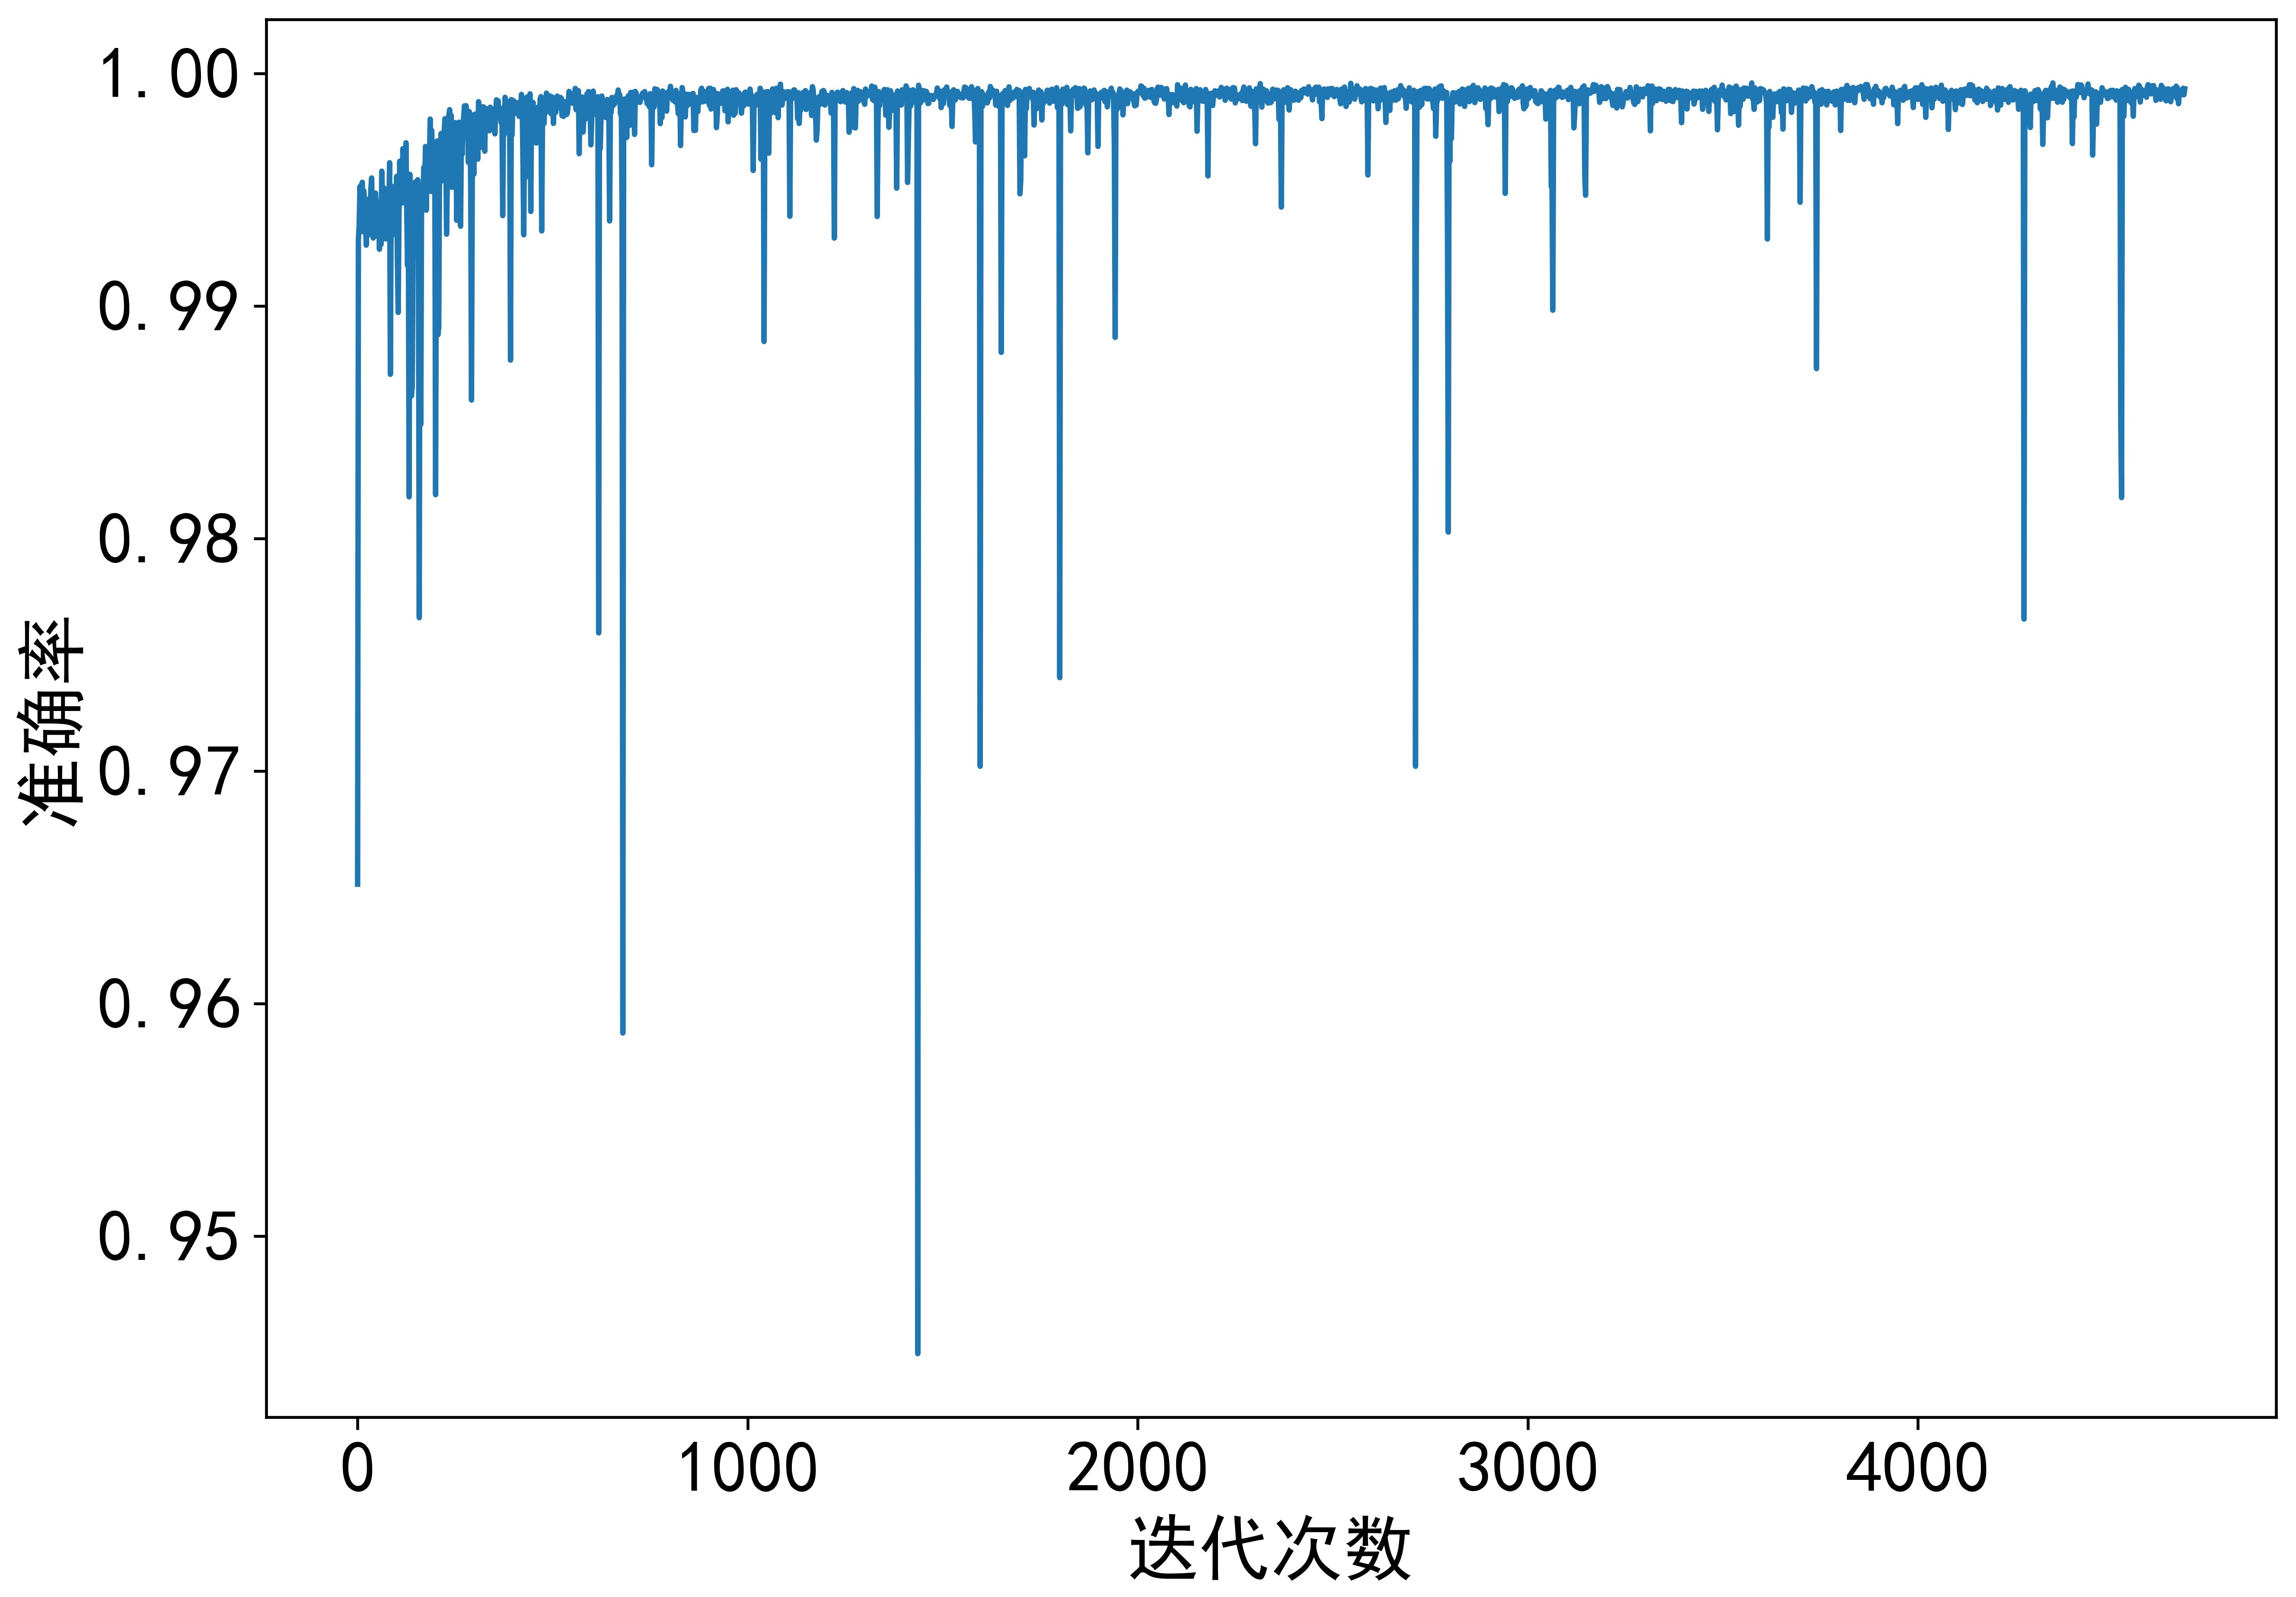
\includegraphics[width=1\linewidth]{figure/chap3/acc.jpg}    
		\caption*{(b) 像素准确率随迭代次数的变化}
		\label{fig:freq}
	\end{minipage}
	\bicaption{训练损失和像素准确率随迭代次数的变化}
	{Training loss and pixel accuracy varied with the number of iterations}%n张图片共享的说明
	\label{fig:train_progress}
	\end{figure}
\subsection{实验结果分析}
\subsubsection{评价指标}
	为了评估线虫轮廓前景分割网络的分割性能,需要一些量化指标来量化分割的结果。本文采用的三个
	量化指标分别为:过分割率(Over Segmentation,OR)、欠分割率(Under Segmentation,UR)以及总体
	分割误差率(Overall Error Rate,ER)\cite{Liu2006Set}。分别由公式\ref{eq:OR}、\ref{eq:UR}和\ref{eq:ER}计算。
	其中$Q_p$表示目标像素被误分类为背景像素的数目,$U_p$为背景像素被误分类为目标像素的数目,$D_n$表示背景像素点
	的数目,$D_p$表示目标像素点的数目。
		\begin{equation}
		OR = Q_p/D_p \label{eq:OR}
		\end{equation}
		\begin{equation}
		UR = U_p/D_n \label{eq:UR}
		\end{equation}
		\begin{equation}
		ER = (Q_p+U_p)/(D_p+D_n)\label{eq:ER}
		\end{equation}
\subsubsection{分割效果对比}
	为了比较分析不同算法的前景轮廓分割效果,本小节我们将本章提出的基于条件随机场的卷积分割算法与传统的
	前景轮廓提取方法进行了对比。图\ref{fig:comp_res}显示了不同算法的分割结果。从图中可以看出基于模糊C均值聚类的
	分割方法和基于阈值分割的OTSU算法的分割结果存在大量的像素分类错误,从原图像可以看出,图像的底部部分的亮度
	较高,但应该属于背景像素,这两种基于像素的分割方法都将这些区域分类为前景像素。另一方面,从原图可以看出线虫的轮廓中心处的
	亮度较低,这两种算法都将这些区域的像素分类为背景,造成了线虫轮廓的不连续以及存在孔洞。虽然经过后处理步骤
	可以针对单张图像过滤掉非线虫轮廓,以及运用形态学图像处理技术可以消除掉线虫轮廓中的空洞和不连续等缺陷,但在
	线虫视频的自动化分析任务中,由于每一帧图像的噪声情况都不一样,因此很难确定一个全局的阈值。 基于高斯混合模型的
	背景减除方法虽然比基于阈值的分割方法和基于聚类的分割方法分割结果有很大的改善,但线虫的轮廓依然存在不连续的
	情况。基于背景减除的分割方法最大的不足在于其只能针对背景固定的视频,因此这种分割具有很大的局限性。
	图\ref{fig:comp_res}(f)是本文不带条件随机场模块的卷积网络(去掉CRF模块,同时用$1\times1$的卷积将特征的
	通道数变为1作为网络的输出)分割的结果。
	从图中可以看出去掉CRF模块后,卷积分割网络由于没有考虑到空间中相邻像素的相关性,从而导致线虫轮廓的不连续,
	分割性能较差。而条件随机场模块能够显著的改善线虫前景轮廓分割中的不连续等情况,与以上的方法相比,其分割性能
	要优于其他的方法,而且其分割的性能不依赖于超参数的选择,具有很好的鲁棒性。
	
\begin{figure}[!htp]
	  \centering

	  \begin{subfigure}{\linewidth}
		\centering
		\begin{minipage}[b]{\linewidth}
		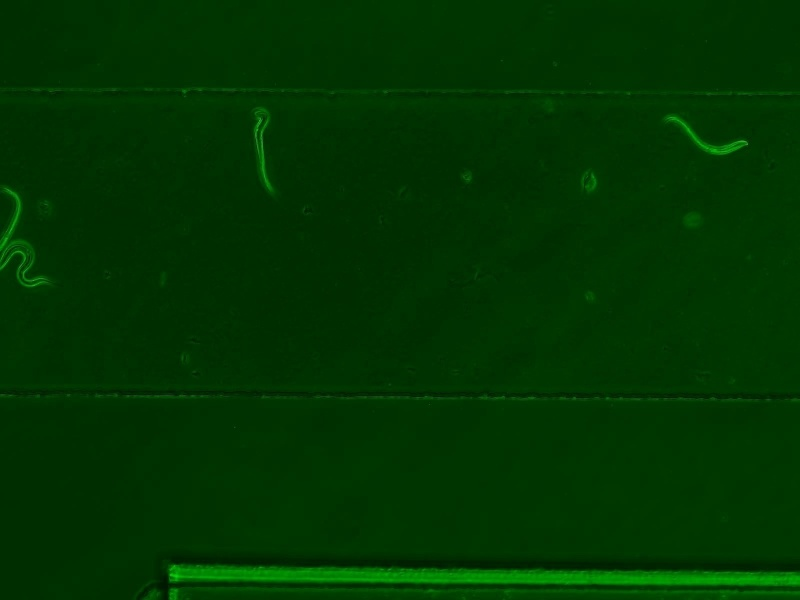
\includegraphics[width=0.33\linewidth,natwidth=800,natheight=600]{figure/chap3/img/441.orgin.851.jpg}
		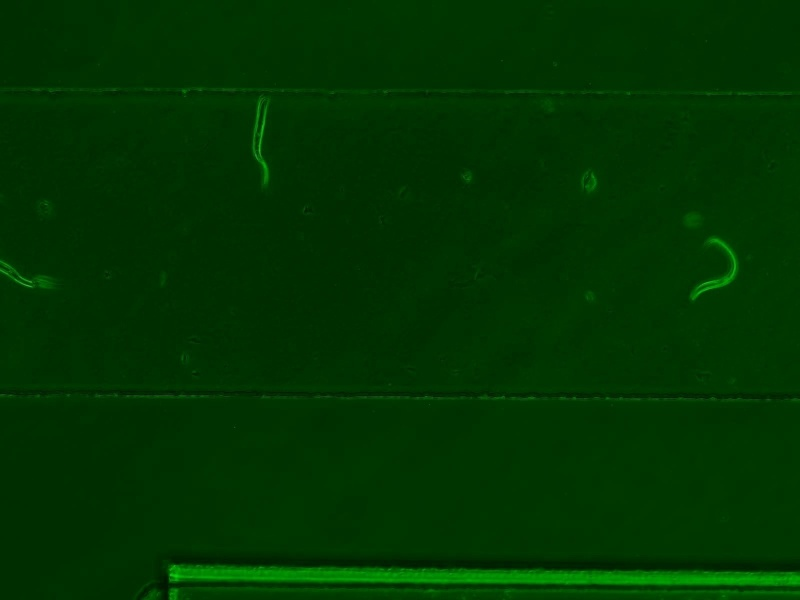
\includegraphics[width=0.33\linewidth,natwidth=800,natheight=600]{figure/chap3/img/441.orgin.1051.jpg}
		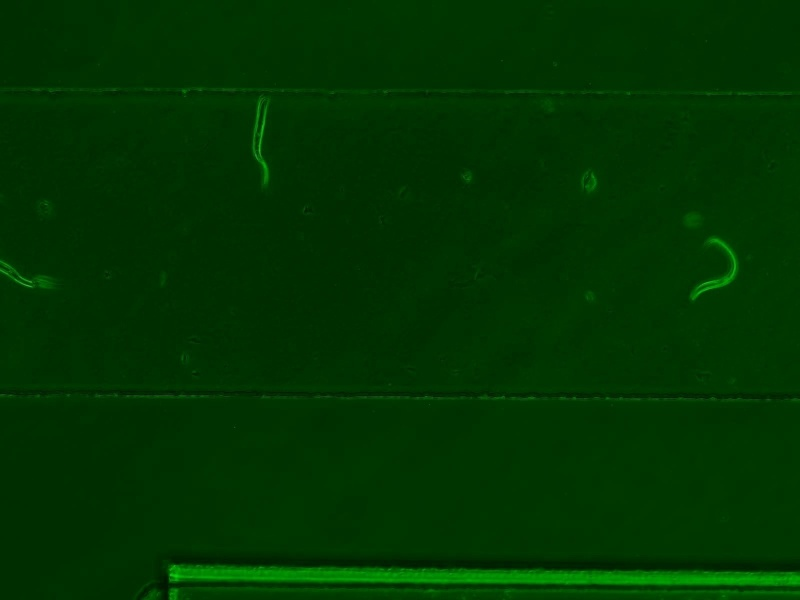
\includegraphics[width=0.33\linewidth,natwidth=800,natheight=600]{figure/chap3/img/441.orgin.1051.jpg}
		\end{minipage}
		\caption{线虫原图像}
	  \end{subfigure}

	 \begin{subfigure}{\linewidth}
		\centering
		\begin{minipage}[b]{\linewidth}
		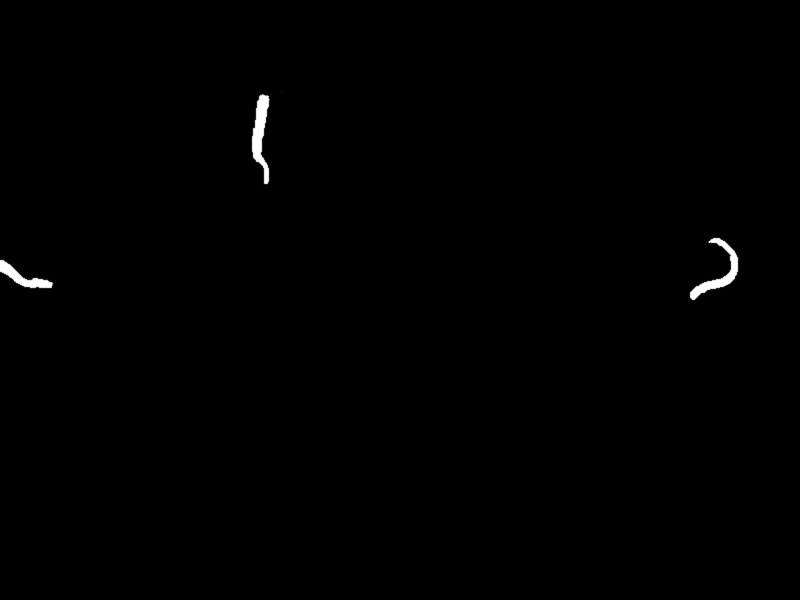
\includegraphics[width=0.33\linewidth,natwidth=800,natheight=600]{figure/chap3/label/441.orgin.1051.jpg}
		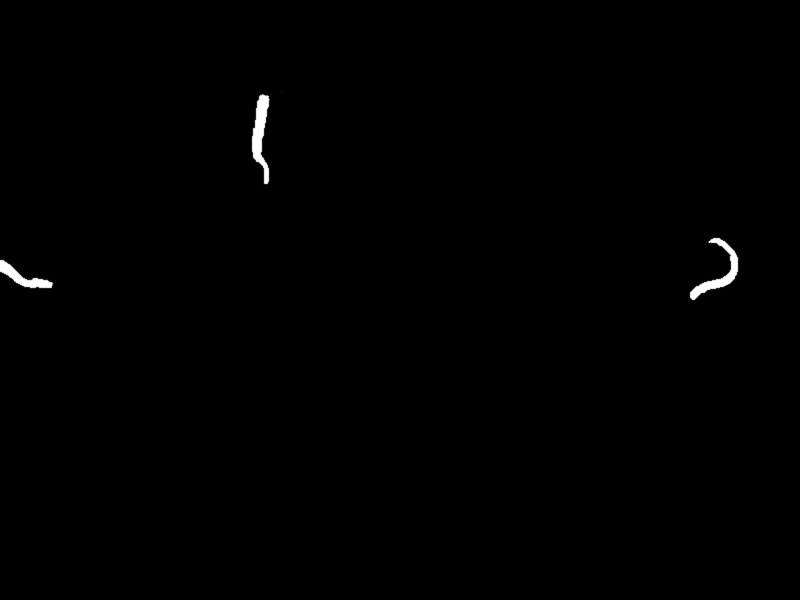
\includegraphics[width=0.33\linewidth,natwidth=800,natheight=600]{figure/chap3/label/441.orgin.1051.jpg}
		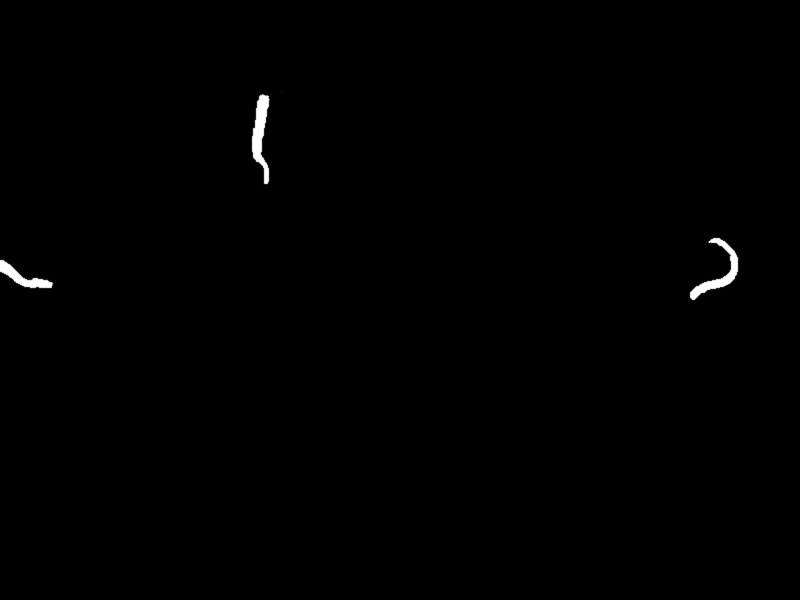
\includegraphics[width=0.33\linewidth,natwidth=800,natheight=600]{figure/chap3/label/441.orgin.1051.jpg}
		\end{minipage}
		\caption{分割标签}
	  \end{subfigure}

	 \begin{subfigure}{\linewidth}
		\centering
		\begin{minipage}[b]{\linewidth}
		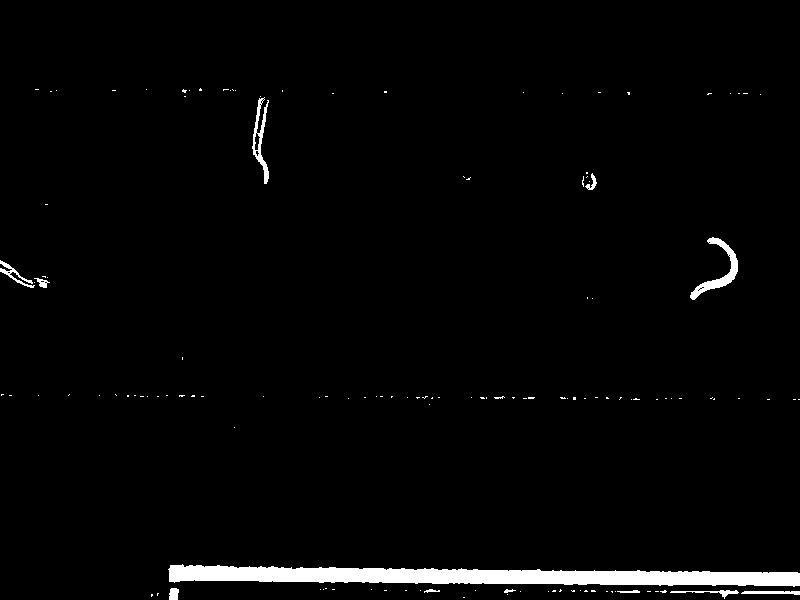
\includegraphics[width=0.33\linewidth,natwidth=800,natheight=600]{figure/chap3/test_otsu/441.orgin.1051.jpg}
		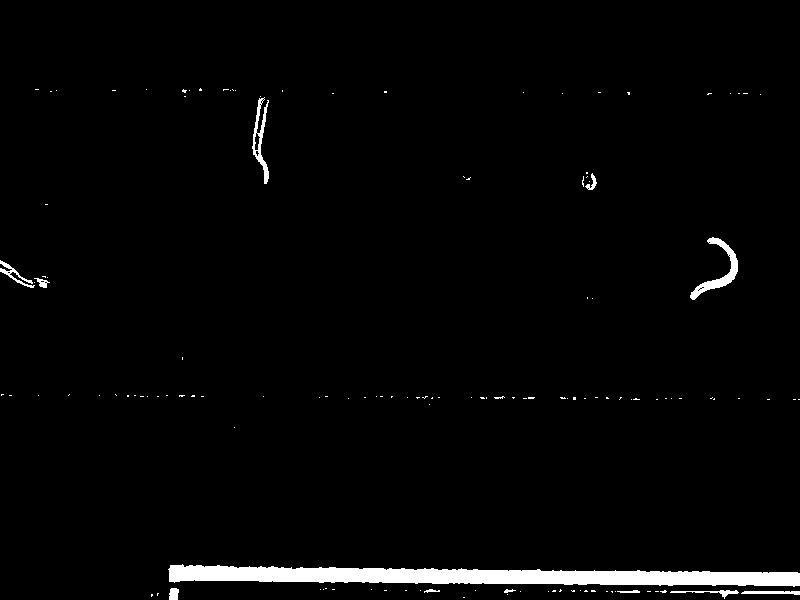
\includegraphics[width=0.33\linewidth,natwidth=800,natheight=600]{figure/chap3/test_otsu/441.orgin.1051.jpg}
		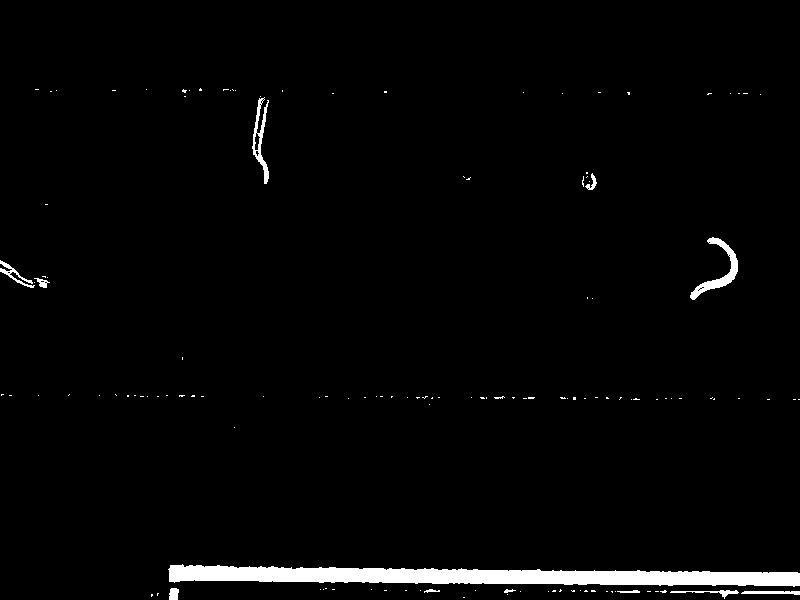
\includegraphics[width=0.33\linewidth,natwidth=800,natheight=600]{figure/chap3/test_otsu/441.orgin.1051.jpg}
		\end{minipage}
		\caption{OTSU阈值分割算法结果}
	  \end{subfigure}

	 \begin{subfigure}{\linewidth}
		\centering
		\begin{minipage}[b]{\linewidth}
		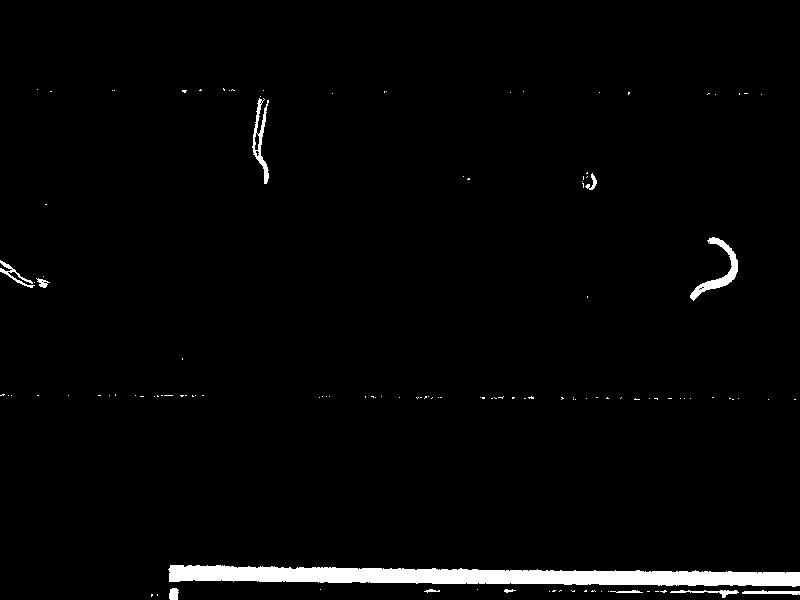
\includegraphics[width=0.33\linewidth,natwidth=800,natheight=600]{figure/chap3/test_fcm/441.orgin.1051.jpg}
		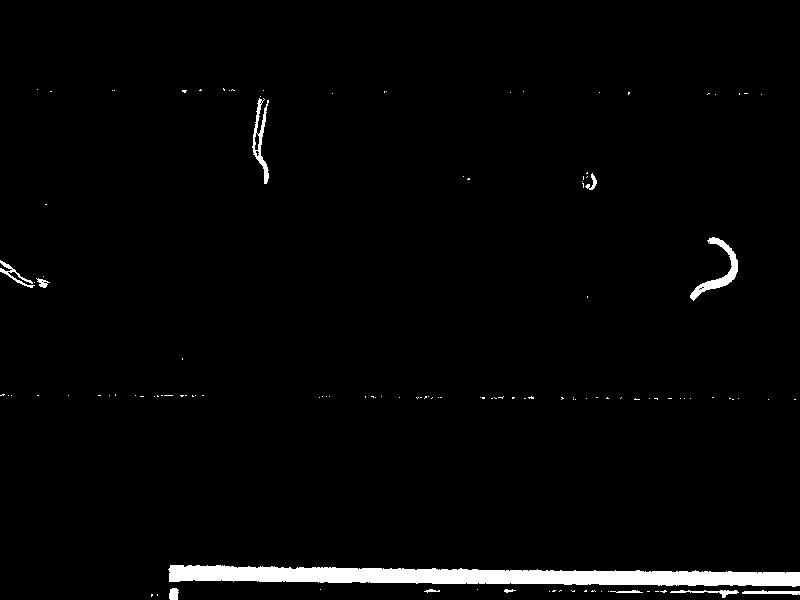
\includegraphics[width=0.33\linewidth,natwidth=800,natheight=600]{figure/chap3/test_fcm/441.orgin.1051.jpg}
		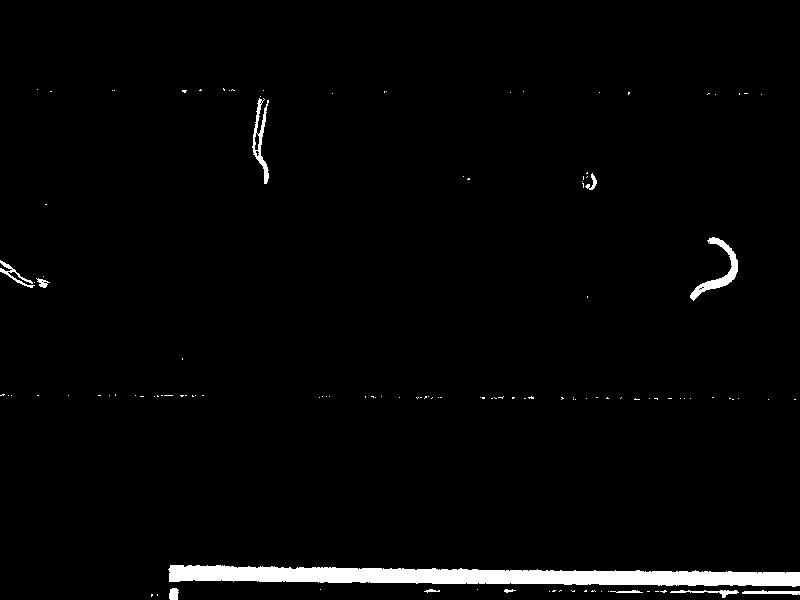
\includegraphics[width=0.33\linewidth,natwidth=800,natheight=600]{figure/chap3/test_fcm/441.orgin.1051.jpg}
		\end{minipage}
		\caption{模糊C均值聚类算法分割结果}
	  \end{subfigure}

	  \begin{subfigure}{\linewidth}
		\centering
		\begin{minipage}[b]{\linewidth}
		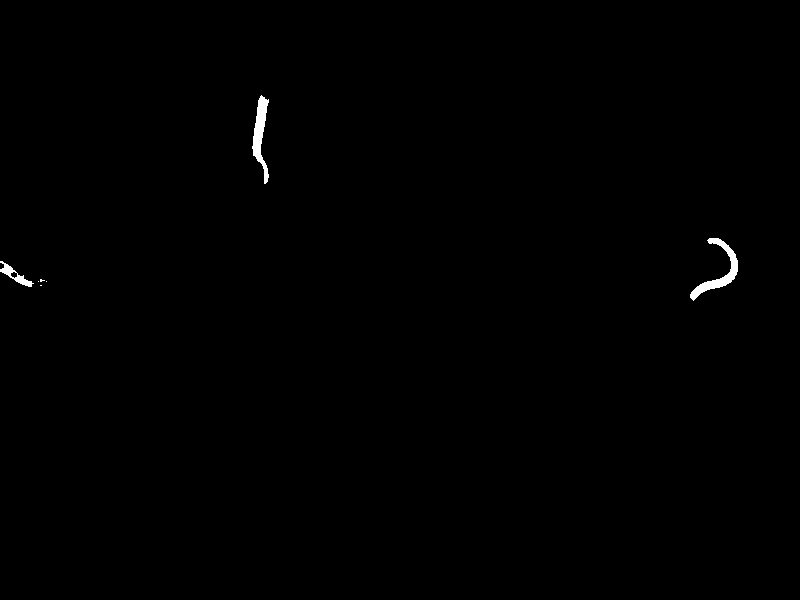
\includegraphics[width=0.33\linewidth,natwidth=800,natheight=600]{figure/chap3/test_bksub/441.orgin.1051.jpg}
		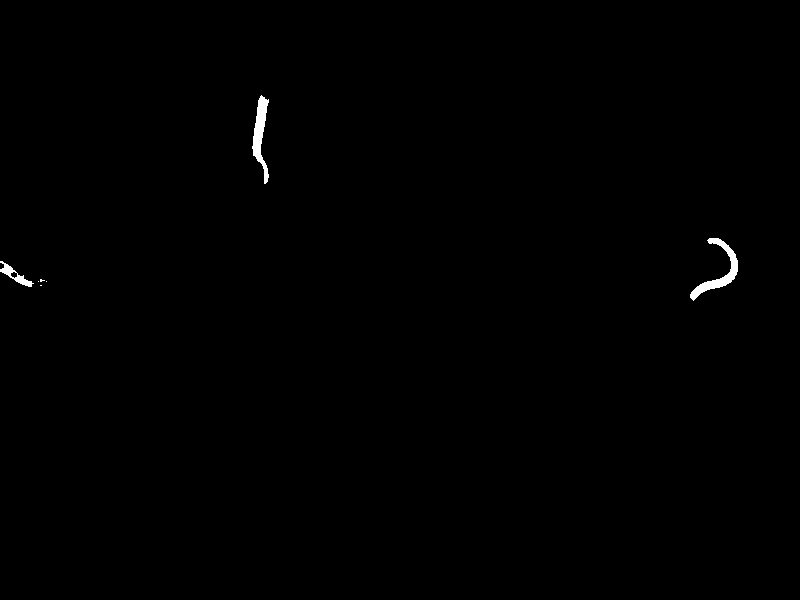
\includegraphics[width=0.33\linewidth,natwidth=800,natheight=600]{figure/chap3/test_bksub/441.orgin.1051.jpg}
		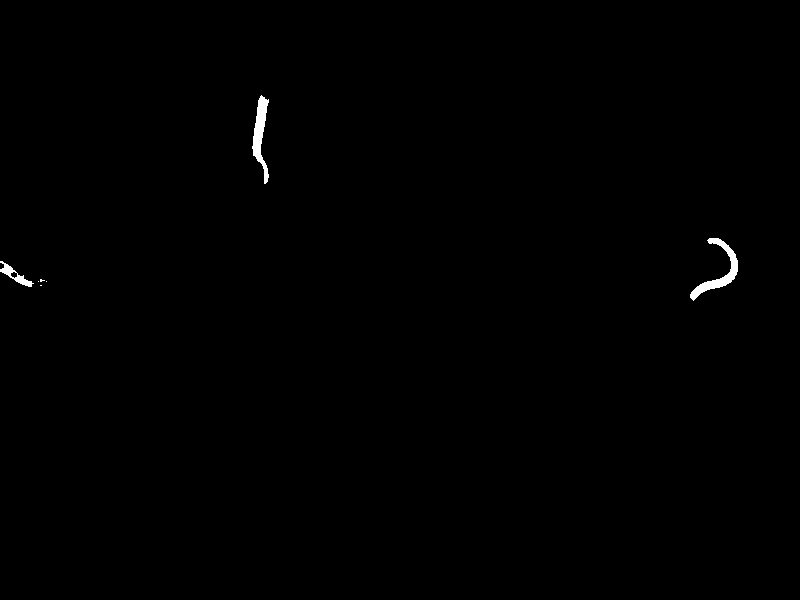
\includegraphics[width=0.33\linewidth,natwidth=800,natheight=600]{figure/chap3/test_bksub/441.orgin.1051.jpg}
		\end{minipage}
		\caption*{(e)混合高斯背景建模的分割算法结果}
	  \end{subfigure}
\end{figure}
\begin{figure}[!htp]
	\addtocounter{subfigure}{5}
		\centering
		\ContinuedFloat
	  \begin{subfigure}{\linewidth}
		\centering
		\begin{minipage}[b]{\linewidth}
		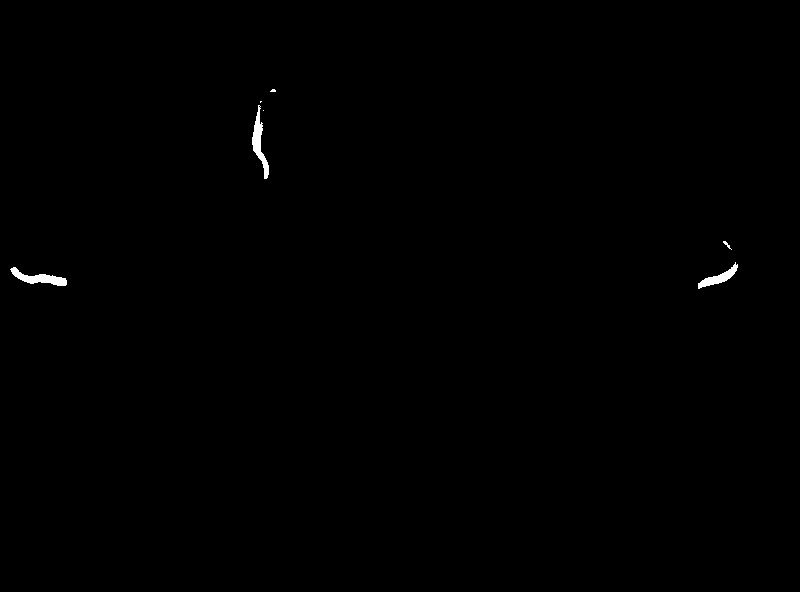
\includegraphics[width=0.33\linewidth,natwidth=800,natheight=600]{figure/chap3/test2/441.orgin.1051.jpg}
		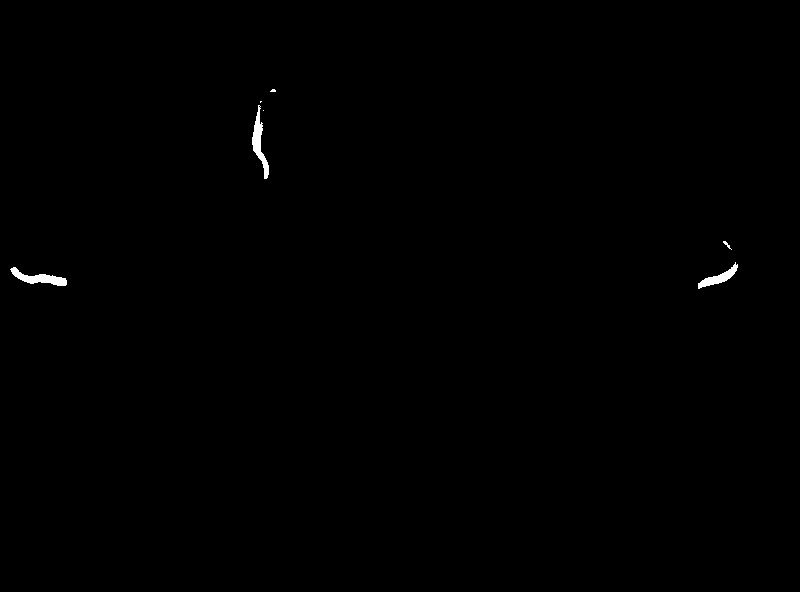
\includegraphics[width=0.33\linewidth,natwidth=800,natheight=600]{figure/chap3/test2/441.orgin.1051.jpg}
		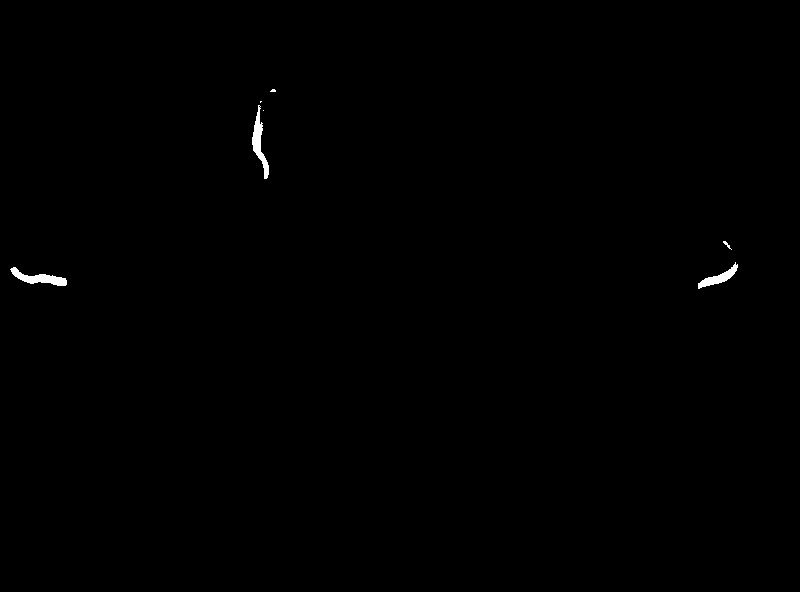
\includegraphics[width=0.33\linewidth,natwidth=800,natheight=600]{figure/chap3/test2/441.orgin.1051.jpg}
		\end{minipage}
		\caption*{(f)本文算法分割结果(没有条件随机场模块)}
	  \end{subfigure}

	  \begin{subfigure}{\linewidth}
		\centering
		\begin{minipage}[b]{\linewidth}
		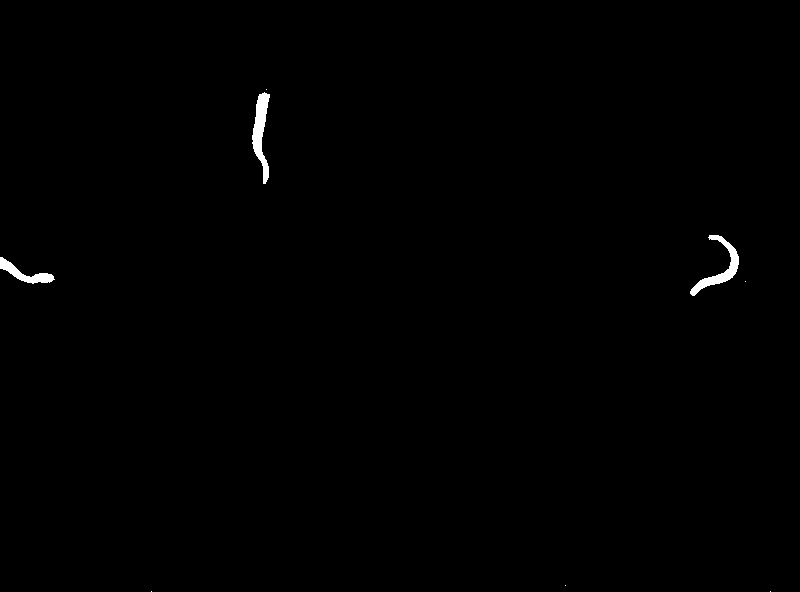
\includegraphics[width=0.33\linewidth,natwidth=800,natheight=600]{figure/chap3/test1/441.orgin.1051.jpg}
		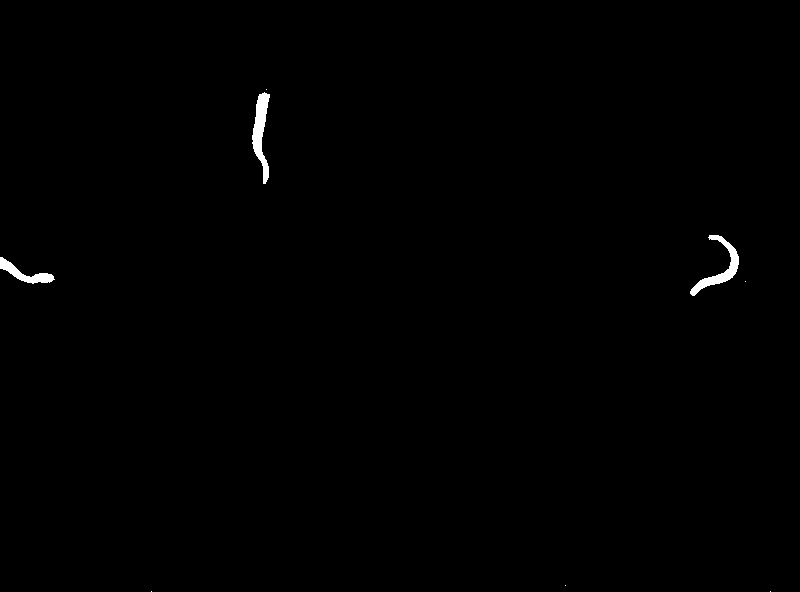
\includegraphics[width=0.33\linewidth,natwidth=800,natheight=600]{figure/chap3/test1/441.orgin.1051.jpg}
		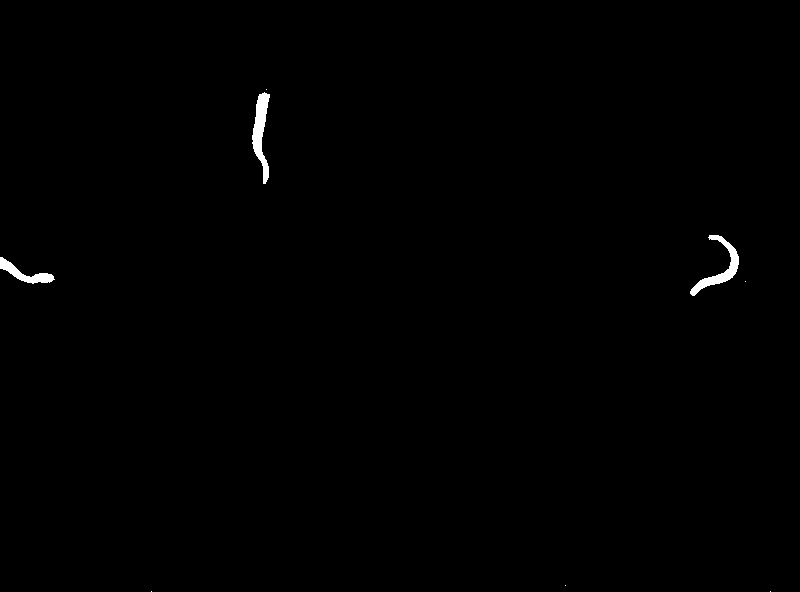
\includegraphics[width=0.33\linewidth,natwidth=800,natheight=600]{figure/chap3/test1/441.orgin.1051.jpg}
		\end{minipage}
		\caption*{(g)本文算法分割结果}
	  \end{subfigure}
	  \bicaption{不同分割算法的分割结果}{The result of different segmentation methods}
	  \label{fig:comp_res}
\end{figure}
\subsubsection{分割性能的量化分析}
	\begin{table}[htbp]
	\centering
	\bicaption[指向一个表格的表目录索引]
    {不同分割方法的性能比较}
    {Performance comparison of different segmentation methods}
	\label{tab:metrics}
	\begin{tabular}{>{\centering}p{80pt}>{\raggedleft\arraybackslash}p{60pt}>{\raggedleft\arraybackslash}p{60pt}>{\raggedleft\arraybackslash}p{60pt}}
	\toprule
	算法&过分割率&欠分割率&总体误差\\
	\midrule
	本文算法 &12.29\% &0.01\% & 0.11\% \\
	本文算法\\(无CRF模块)&26.93\% & 0.03\% &0.17\% \\
	背景减除  &19.55\% & 0.02\%& 0.12\% \\
	OTSU算法 &26.62\% & 2.12\% & 2.25\% \\
	FCM 算法 &27.41\% & 2.15\% & 2.28\% \\
	\bottomrule
	\end{tabular}
	\end{table}
	为了定量的分析不同分割算法的性能,本文采用了三种性能指标对不同算法在测试集上分割的结果进行量化如表\ref{tab:metrics}所示。
	从表中可以看出基于阈值分割的OTSU算法和基于聚类的FCM算法在过分割率、欠分割率以及总体误差三个指标上均表现较差。
	另外,没有使用CRF的卷积分割网络在三个指标上的表现均弱于基于背景减除的分割方法。但在卷积网络后端加入CRF模块后,网络的分割性能
	有了很大的提升,其分割性能要优于其他的分割算法,总体的像素误差下降到$0.11\%$。
	
\section{本章小结}
	本章首先介绍了线虫图像总体流程包括:前景轮廓分割、轮廓解析、轮廓跟踪和特征提取等步骤。在介绍的
	前景分割算法之前,先分类回顾了传统的图像分割方法。然后介绍了卷积网络的原理并介绍了两种正则化方法。紧接着
	重点介绍本文提出的基于条件随机场模型的全卷积分割架构的设计。最后是网络的训练和实验结果分析,实验表明,
	本章提出的分割算法与传统的图像分割算法相比,在线虫前景轮廓分割任务中具有更好的分割性能。
	